%%%%%%%%%%%%%%%%%%%%%%%%%%%%%%%%%%%%%%%%%%%%%%%%%%%%%%%%%%%%%%%%%%%%%%%%%%%%%%%%
%% Plantilla de memoria en LaTeX para la ETSIT - Universidad Rey Juan Carlos
%%
%% Por Gregorio Robles <grex arroba gsyc.urjc.es>
%%     Grupo de Sistemas y Comunicaciones
%%     Escuela Técnica Superior de Ingenieros de Telecomunicación
%%     Universidad Rey Juan Carlos
%% (muchas ideas tomadas de Internet, colegas del GSyC, antiguos alumnos...
%%  etc. Muchas gracias a todos)
%%
%% La última versión de esta plantilla está siempre disponible en:
%%     https://github.com/gregoriorobles/plantilla-memoria
%%
%% Para obtener PDF, ejecuta en la shell:
%%   make
%% (las imágenes deben ir en PNG o JPG)

%%%%%%%%%%%%%%%%%%%%%%%%%%%%%%%%%%%%%%%%%%%%%%%%%%%%%%%%%%%%%%%%%%%%%%%%%%%%%%%%

\documentclass[a4paper, 12pt]{book}
%\usepackage[T1]{fontenc}

\usepackage[a4paper, left=2.5cm, right=2.5cm, top=3cm, bottom=3cm]{geometry}
\usepackage{times}
\usepackage[utf8]{inputenc}
\usepackage[spanish]{babel} % Comenta esta línea si tu memoria es en inglés
\usepackage{url}
%\usepackage[dvipdfm]{graphicx}
\usepackage{graphicx}
\usepackage{float}  %% H para posicionar figuras
\usepackage[nottoc, notlot, notlof, notindex]{tocbibind} %% Opciones de índice
\usepackage{latexsym}  %% Logo LaTeX

\usepackage{subfig}

\usepackage{array}

\title{Memoria del Proyecto}
\author{Nombre del autor}

\renewcommand{\baselinestretch}{1.5}  %% Interlineado

\begin{document}

\renewcommand{\refname}{Bibliografía}  %% Renombrando
\renewcommand{\appendixname}{Apéndice}

%%%%%%%%%%%%%%%%%%%%%%%%%%%%%%%%%%%%%%%%%%%%%%%%%%%%%%%%%%%%%%%%%%%%%%%%%%%%%%%%
% PORTADA

\begin{titlepage}
\begin{center}
\includegraphics[scale=0.6]{img/URJ_logo_Color_POS.png}

\vspace{1.75cm}

\LARGE
ESCUELA DE INGENIERÍA DE FUENLABRADA
\vspace{1cm}

\LARGE
GRADO EN INGENIERÍA EN SISTEMAS AUDIOVISUALES Y MULTIMEDIA

\vspace{1cm}
\LARGE
\textbf{TRABAJO FIN DE GRADO}

\vspace{2cm}

\Large
DR.SCRATCHJR \\ 
ANÁLISIS AUTOMÁTICO DE PROYECTOS SCRATCHJR

\vspace{2cm}

\large
Autor : Sergio Pérez Mazadiego \\
Tutor : Dr. Gregorio Robles\\
\vspace{1cm}

\large
Curso académico 2022/2023

\end{center}
\end{titlepage}

\newpage
\mbox{}
\thispagestyle{empty} % para que no se numere esta pagina


%%%%%%%%%%%%%%%%%%%%%%%%%%%%%%%%%%%%%%%%%%%%%%%%%%%%%%%%%%%%%%%%%%%%%%%%%%%%%%%%
%%%% Para firmar
\clearpage
\pagenumbering{gobble}
\chapter*{}

\vspace{-4cm}
\begin{center}
\LARGE
\textbf{Trabajo Fin de Grado}

\vspace{1cm}
\large
Dr.ScratchJr, Análisis Automático de Proyectos ScratchJr

\vspace{1cm}
\large
\textbf{Autor :} Sergio Pérez Mazadiego \\
\textbf{Tutor :} Dr. Gregorio Robles

\end{center}

\vspace{1cm}
La defensa del presente Proyecto Fin de Carrera se realizó el día \qquad$\;\,$ de \qquad\qquad\qquad\qquad \newline de 2023, siendo calificada por el siguiente tribunal:


\vspace{0.5cm}
\textbf{Presidente:}

\vspace{1.2cm}
\textbf{Secretario:}

\vspace{1.2cm}
\textbf{Vocal:}


\vspace{1.2cm}
y habiendo obtenido la siguiente calificación:

\vspace{1cm}
\textbf{Calificación:}


\vspace{1cm}
\begin{flushright}
Fuenlabrada, a \qquad$\;\,$ de \qquad\qquad\qquad\qquad de 2023
\end{flushright}

%%%%%%%%%%%%%%%%%%%%%%%%%%%%%%%%%%%%%%%%%%%%%%%%%%%%%%%%%%%%%%%%%%%%%%%%%%%%%%%%
%%%% Dedicatoria

\chapter*{}
\pagenumbering{Roman} % para comenzar la numeración de paginas en numeros romanos
\begin{flushright}
\textit{Dedicado a \\
mi familia y amigos}
\end{flushright}

%%%%%%%%%%%%%%%%%%%%%%%%%%%%%%%%%%%%%%%%%%%%%%%%%%%%%%%%%%%%%%%%%%%%%%%%%%%%%%%%
%%%% Agradecimientos

\chapter*{Agradecimientos}
%\addcontentsline{toc}{chapter}{Agradecimientos} % si queremos que aparezca en el índice
\markboth{AGRADECIMIENTOS}{AGRADECIMIENTOS} % encabezado 

Agradecer a mis padres por el apoyo, la confianza y sobre todo por servirme lo que ellos no han podido tener, esa comodidad y estabilidad que siempre ha hecho que pueda tener una vida sin preocupaciones y llena de oportunidades.


%%%%%%%%%%%%%%%%%%%%%%%%%%%%%%%%%%%%%%%%%%%%%%%%%%%%%%%%%%%%%%%%%%%%%%%%%%%%%%%%
%%%% Resumen

\chapter*{Resumen}
%\addcontentsline{toc}{chapter}{Resumen} % si queremos que aparezca en el índice
\markboth{RESUMEN}{RESUMEN} % encabezado

Este trabajo final de grado consiste en el desarrollo de una herramienta que analice proyectos de ScratchJr, un lenguaje de programación para niños de edades entre 5 y 7.  
La idea surge con el objetivo de hacer una herramienta similar a Dr.Scratch, que es una aplicación web que analiza proyectos de Scratch, otro lenguaje de iniciación a la programación. 

\vspace{5mm}

Como resultado del trabajo fin de grado se ha creado una aplicación web llamada Dr.ScratchJr para que profesores o padres de niños que usen ScratchJr, puedan subir sus proyectos y vean un análisis de éstos.
En el análisis de un proyecto se estudia la variabilidad en el uso de bloques, los malos hábitos que contiene, la creatividad y otros datos que podrían llegar a ser de interés como el total de páginas o personajes que se usan en él. 
La aplicación web ofrece la posibilidad de analizar uno, o varios proyectos a la vez, o crear una cuenta en la aplicación para poder almacenar los análisis de proyectos y tener una gestión de sus autores. 
En ambos casos la aplicación dispone de la opción de exportar los datos de los análisis en formato CSV.

\vspace{5mm}

Las tecnologías que se han empleado son en el lado del servidor el software de desarrollo Django en el que se utiliza Python, y Bootstrap en el lado del cliente en el que se utiliza HTML, CSS y JavaScript.

%%%%%%%%%%%%%%%%%%%%%%%%%%%%%%%%%%%%%%%%%%%%%%%%%%%%%%%%%%%%%%%%%%%%%%%%%%%%%%%%
%%%% Resumen en inglés

\chapter*{Summary}
%\addcontentsline{toc}{chapter}{Summary} % si queremos que aparezca en el índice
\markboth{SUMMARY}{SUMMARY} % encabezado

Here comes a translation of the ``Resumen'' into English. 
Please, double check it for correct grammar and spelling.
As it is the translation of the ``Resumen'', which is supposed to be written at the end, this as well should be filled out just before submitting.


%%%%%%%%%%%%%%%%%%%%%%%%%%%%%%%%%%%%%%%%%%%%%%%%%%%%%%%%%%%%%%%%%%%%%%%%%%%%%%%%
%%%%%%%%%%%%%%%%%%%%%%%%%%%%%%%%%%%%%%%%%%%%%%%%%%%%%%%%%%%%%%%%%%%%%%%%%%%%%%%%
% ÍNDICES %
%%%%%%%%%%%%%%%%%%%%%%%%%%%%%%%%%%%%%%%%%%%%%%%%%%%%%%%%%%%%%%%%%%%%%%%%%%%%%%%%

% Las buenas noticias es que los índices se generan automáticamente.
% Lo único que tienes que hacer es elegir cuáles quieren que se generen,
% y comentar/descomentar esa instrucción de LaTeX.

%%%% Índice de contenidos
\tableofcontents 
%%%% Índice de figuras
\cleardoublepage
%\addcontentsline{toc}{chapter}{Lista de figuras} % para que aparezca en el indice de contenidos
\listoffigures % indice de figuras
%%%% Índice de tablas
%\cleardoublepage
%\addcontentsline{toc}{chapter}{Lista de tablas} % para que aparezca en el indice de contenidos
%\listoftables % indice de tablas


%%%%%%%%%%%%%%%%%%%%%%%%%%%%%%%%%%%%%%%%%%%%%%%%%%%%%%%%%%%%%%%%%%%%%%%%%%%%%%%%
%%%%%%%%%%%%%%%%%%%%%%%%%%%%%%%%%%%%%%%%%%%%%%%%%%%%%%%%%%%%%%%%%%%%%%%%%%%%%%%%
% INTRODUCCIÓN %
%%%%%%%%%%%%%%%%%%%%%%%%%%%%%%%%%%%%%%%%%%%%%%%%%%%%%%%%%%%%%%%%%%%%%%%%%%%%%%%%

\cleardoublepage
\chapter{Introducción}
\label{chap:intro} % etiqueta para poder referenciar luego en el texto con~\ref{chap:intro}
\pagenumbering{arabic} % para empezar la numeración de página con números

Las habilidades de programación son cada vez  más necesarias que se empiecen a trabajar en las aulas desde los inicios en la educación, igual que se enseña la lengua, las matemáticas, la historia, puesto que favorecen la estructuración del pensamiento crítico y la lógica, esenciales en la resolución de problemas.
Difícilmente se consigue enseñar a un niño de unos 5 o 6 años a que escriba código de programación.
Pero sí es posible que comience a familiarizarse con el mundo de la programación y su lenguaje general sin que se dé cuenta de una manera lúdica y al mismo tiempo formativa.
Como en las primeras edades sus capacidades lectoescritoras todavía están formándose, por medio de herramientas vinculadas a elementos visuales como juegos, puzzles o aventuras, podemos arrancar el desarrollo del pensamiento computacional recurriendo a su creatividad. Algunas herramientas que podemos encontrar son las aplicaciones Kodable\footnote{\url{https://www.kodable.com/}}, Bit by bit\footnote{\url{http://rikaigames.com/bitbybit/}}, Codekarts\footnote{\url{https://civat.es/app/code-karts/}} y ScratchJr\footnote{\url{https://www.scratchjr.org/}}. 

De esta última, ScratchJr (que se introduce en detalle en la Sección~\ref{sec:scratchJr}), es donde parte este proyecto.
ScratchJr está basada en Scratch pero con su interfaz y lenguaje de programación rediseñados para niños más pequeños.
En la URJC se desarrolló la herramienta Dr.Scratch que permite a los usuarios de Scratch analizar sus proyectos y medir sus capacidades de programación cuantificadas por medidores de habilidades de pensamiento computacional.
De esta misma idea surge Dr.ScratchJr.
Pero debido a que los usuarios de ScratchJr, al ser demasiado pequeños, no tienen todavía la capacidad de poder autoevaluar sus propios proyectos, el objetivo principal de la herramienta Dr.ScratchJr es facilitar a los profesores el proceso de enseñanza de sus alumnos.
Con ella, los profesores pueden analizar los proyectos que hayan hecho sus alumnos en ScratchJr.

\section{Estructura de la memoria}
\label{sec:estructura}

La memoria del trabajo está estructurada en los siguientes capítulos:

\begin{itemize}
    \item Capítulo~\ref{chap:intro}: \textbf{Introducción}.
    Capítulo actual donde se presenta el tema del que va a tratar el proyecto y se marca la estructura de la memoria.
    \item Capítulo~\ref{chap:objetivos}: \textbf{Objetivos}. 
    Partiendo del objetivo general, se plantean los objetivos que se han ido marcando para la realización del proyecto.
    \item Capítulo~\ref{chap:estado}: \textbf{Estado del arte}. 
    Aparecen pequeñas descripciones de las tecnologías utilizadas en la realización de la herramienta Dr.ScratchJr.
    \item Capítulo~\ref{chap:implementacion}: \textbf{Diseño e implementación}. 
    Se explica la arquitectura general de la herramienta Dr.ScratchJr, el algoritmo del tratamiento de datos para realizar el análisis y la vista de la aplicación web.
    \item Capítulo~\ref{chap:experimentos}: \textbf{Experimentos, validación y resultados}. 
    Se realizan pruebas con un proyecto de test para validar que la herramienta detecta todos los datos a analizar correctamente, una pequeña comprobación de la correcta carga de varios proyectos y otra de la exportación de los datos en CSV.
    \item Capítulo~\ref{chap:conclusiones}: \textbf{Conclusiones}. 
    Se exponen varias secciones donde se trata la consecución de los objetivos, las asignaturas del Grado que me han servido para la realización del proyecto, aquello que he aprendido gracias a la elaboración de dicho proyecto y algunas ideas de la herramienta para futuras mejoras.
    
\end{itemize}



%%%%%%%%%%%%%%%%%%%%%%%%%%%%%%%%%%%%%%%%%%%%%%%%%%%%%%%%%%%%%%%%%%%%%%%%%%%%%%%%
%%%%%%%%%%%%%%%%%%%%%%%%%%%%%%%%%%%%%%%%%%%%%%%%%%%%%%%%%%%%%%%%%%%%%%%%%%%%%%%%
% OBJETIVOS %
%%%%%%%%%%%%%%%%%%%%%%%%%%%%%%%%%%%%%%%%%%%%%%%%%%%%%%%%%%%%%%%%%%%%%%%%%%%%%%%%

\cleardoublepage % empezamos en página impar
\chapter{Objetivos} % título del capítulo (se muestra)
\label{chap:objetivos} % identificador del capítulo (no se muestra, es para poder referenciarlo)

\section{Objetivo general} % título de sección (se muestra)
\label{sec:objetivo-general} % identificador de sección (no se muestra, es para poder referenciarla)

El objetivo principal de este proyecto es desarrollar una herramienta de análisis similar a Dr.Scratch para ScratchJr.
En Dr.Scratch los usuarios pueden evaluar sus propios proyectos creados con Scratch, pero como los destinatarios de ScratchJr son niños, el objetivo es crear una aplicación web con la función de ser una herramienta para que profesores o padres puedan analizar los proyectos de ScratchJr de los niños.
De esta manera se facilita y agiliza el trabajo de evaluación y poder guiar a los niños a un mayor aprendizaje detectando los errores más frecuentes que suelen darse en la programación.


\section{Objetivos específicos}
\label{sec:objetivos-especificos}

Para cumplir con el objetivo principal ha sido necesario seguir los siguientes objetivos específicos:

\begin{itemize}
    \item Comprender la herramienta DrScratch.
    \item Ampliar y mejorar los conocimientos sobre la creación de aplicaciones web con Django e instalar las tecnologías necesarias para ello.
    \item Examinar la estructura de la aplicación ScratchJr: el uso y funcionamiento, los tipos de bloques y componentes que pueden emplearse y los ficheros que forman un proyecto.
    \item Estudiar el fichero JSON de datos que ScratchJr genera en cada proyecto.
    \item Extraer y almacenar en una base de datos los elementos y datos de los proyectos generados por ScratchJr.
    \item Crear los algoritmos para tratar y adaptar los datos para los distintos criterios del análisis en la aplicación web.
    \item Desarrollar la aplicación web para que se adapte a diferentes dispositivos con distintas resoluciones.
    \item Diseñar un sistema de administración que permita a profesores tener un control de sus alumnos y los análisis de los proyectos de estos.
    \item Implementar un sistema de exportación de archivos con los resultados de los análisis de los proyectos.
    \item Desplegar la aplicación web en un servidor web público.
    
\end{itemize}


%%%%%%%%%%%%%%%%%%%%%%%%%%%%%%%%%%%%%%%%%%%%%%%%%%%%%%%%%%%%%%%%%%%%%%%%%%%%%%%%
%%%%%%%%%%%%%%%%%%%%%%%%%%%%%%%%%%%%%%%%%%%%%%%%%%%%%%%%%%%%%%%%%%%%%%%%%%%%%%%%
% ESTADO DEL ARTE %
%%%%%%%%%%%%%%%%%%%%%%%%%%%%%%%%%%%%%%%%%%%%%%%%%%%%%%%%%%%%%%%%%%%%%%%%%%%%%%%%

\cleardoublepage
\chapter{Estado del arte}
\label{chap:estado}

Para el desarrollo del proyecto se han utilizado una serie de tecnologías ya existentes que se describen a continuación.


\section{ScratchJr}
\label{sec:scratchJr}

ScratchJr~\cite{scratchjr,leidl2017programming} (figura~\ref{fig:scratchjr}) es un lenguaje de programación de iniciación que permite a los niños pequeños crear sus propias historias y juegos interactivos.
Está inspirado en el lenguaje de programación Scratch\footnote{\url{https://scratch.mit.edu/about}} utilizado por millones de jóvenes en todo el mundo.
ScratchJr ha rediseñado tanto la interfaz como el lenguaje de programación para adecuarlo al desarrollo de los niños más pequeños.

\begin{figure}[ht]
  \centering
  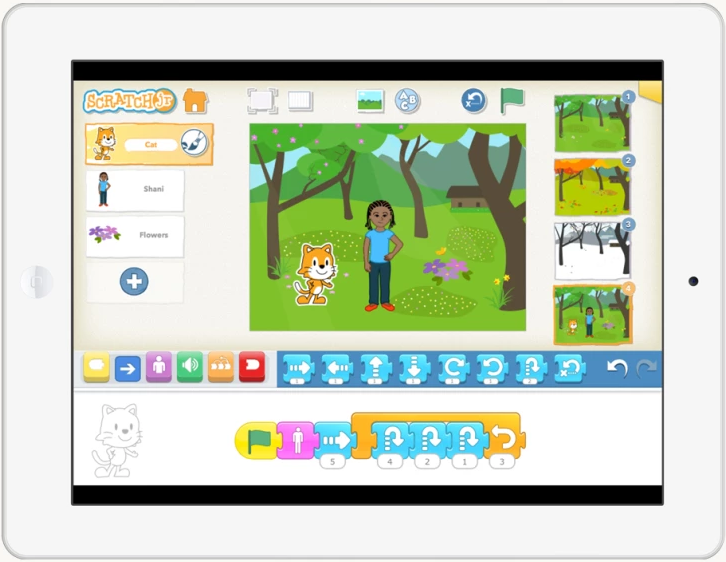
\includegraphics[width=8cm, keepaspectratio]{img/scratchjr.png}
  \caption{Aplicación ScratchJr.}\label{fig:scratchjr}
\end{figure}

\vspace{5mm}
A través de la unión de bloques gráficos de programación, los niños hacen que los personajes se muevan, salten, bailen y canten.
Los niños pueden modificar los personajes o crear nuevos en el editor de dibujos, donde incluso pueden subir sus propias fotos, y luego usar los bloques de programación para hacer que los personajes cobren vida dentro de distintos escenarios.

\vspace{5mm}
Las funciones están cuidadosamente diseñadas para adaptarse al desarrollo cognitivo, personal, social y emocional de los niños.
Estos no sólo aprenden a programar, sino que además desarrollan destrezas que son fundamentales para su desarrollo académico.

\vspace{5mm}
ScratchJr está disponible como una aplicación gratuita para dispositivos iOS y Android.
Además, permite compartir los proyectos creados entre usuarios a través de correo electrónico o AirDrop.

\section{Dr.Scratch}
\label{sec:drscratch}

Por hacer~\cite{moreno2015dr}

\section{Python}
\label{sec:python}

Python~\cite{python} es un lenguaje de programación de alto nivel, interpretado, dinámico, fuertemente tipado y multiplataforma.
Se considera multiparadigma ya que soporta parcialmente la orientación a objetos, programación imperativa y programación funcional, además de otros paradigmas mediante el uso de extensiones.

\vspace{5mm}
Aunque generalmente los programas escritos en Python muestran un tiempo de ejecución mayor respecto a programas en otros lenguajes, para el programador Python requiere un menor tiempo de desarrollo gracias a su sencillez, claridad y versatilidad.

\vspace{5mm}
Está desarrollado bajo una licencia de código abierto, por lo que es de libre uso y distribución.
Lo que supone que además de contar con una gran biblioteca estándar, exista una colección creciente de programas, módulos, paquetes o \emph{frameworks}, disponibles en el Python Package Index\footnote{\url{https://pypi.org/}}.


\section{Django}
\label{sec:django}

Django~\cite{django} es un framework de desarrollo web de alto nivel escrito en Python (sección~\ref{sec:python}).
Se encarga de facilitar la creación de sitios web dinámicos de manera relativamente rápida y con un diseño limpio.
Es de software libre y de código abierto.

\vspace{5mm}
Contiene un número reducido de ficheros y carpetas.
Está basado en el principio DRY (Don't Repeat Yourself o No te repitas) para evitar escribir código duplicado e invertir el menor esfuerzo posible en patrones repetitivos para poderse centrar en la parte creativa.

\vspace{5mm} % DUDA: poner comillas Vista, Plantilla?
Está inspirado por su versatilidad y simpleza en el patrón de arquitectura software MVC (Modelo-Vista-Controlador), pero Django redefine este patrón en Modelo, Vista y Plantilla.
Lo que se llamaría Controlador en un verdadero framework MVC, se llama Vista en Django, y lo que se llamaría Vista, se llama Plantilla.

\begin{itemize}
    \item \textbf{Modelo}: es la capa de abstracción en código (\texttt{models.py}) de la base de datos, manejada como un objeto encargado de la interacción y comunicación con la base de datos.
    \item \textbf{Vista}: es la capa designada a la lógica de la página web, a través de la que pasarán los datos del modelo a la plantilla.
    \item \textbf{Plantilla}: se encarga de presentar al usuario la información disponible en un formato adecuado. 
\end{itemize}

Django incluye una capa de mapeo relacional de objetos (ORM) predeterminada que se puede usar para interactuar con datos de aplicaciones de varias bases de datos relacionales, sin necesidad de conocer los comandos de la base de datos.
Viene con SQLite3 por defecto, pero es posible disponer de otro motor de base de datos como PostgreSQL, MySQL o Oracle.

\vspace{5mm}
Aporta un servidor propio para la parte de desarrollo de una aplicación, pero se puede montar sobre otros servidores para la parte de producción.

\vspace{5mm}
También se toma la seguridad muy en serio y ayuda a los desarrolladores a evitar muchos errores de seguridad comunes, como el método de infiltración de código intruso (SQL injection), las secuencias de comandos en sitios cruzados (Cross-site scripting o XSS), la falsificación de solicitudes entre sitios (Cross Site Request Forgery o CSRF) y el secuestro de clic (Clickjacking).
Además, su sistema de autenticación de usuarios proporciona una forma segura de administrar las cuentas y contraseñas de los usuarios.


\section{Django-registration} 
\label{sec:django-registration}

Django-registration~\cite{Bennett01:django-registration} es una aplicación extensible que proporciona la funcionalidad de registro de usuarios para sitios web con tecnología Django (sección~\ref{sec:django}).

\vspace{5mm}
Aunque casi todos los aspectos del proceso de registro son personalizables, proporciona vistas y mecanismos predefinidos para dos casos de uso comunes:

\begin{itemize}
    \item \textbf{Registro en dos fases:} consiste en el registro inicial seguido de un correo electrónico de confirmación con instrucciones para activar la nueva cuenta.
    \item \textbf{Registro de una fase:} la activación del usuario registrado y el inicio de sesión es inmediato.
\end{itemize}


\section{HTML5 (HyperText Markup Language)} 
\label{sec:html5}

HTML5~\cite{html} es la última versión de HTML, la quinta, lanzada en 2014. Es un lenguaje de marcado que se utiliza para estructurar y desplegar páginas web.

\vspace{5mm}
Ofrece una gran adaptabilidad, una estructuración lógica y facilidad de interpretación.
Un documento HTML se compone en base a etiquetas, también llamadas marcas o tags, con las cuales conseguimos expresar el contenido (elementos) de una página web (cabecera, cuerpo, encabezados, párrafos, archivos…).
Los elementos tienen dos propiedades básicas: atributos y contenido.
Los atributos del elemento están contenidos en la etiqueta de inicio del elemento y el contenido está ubicado entre esta etiqueta y la de cierre.

\vspace{5mm}
Es multiplataforma siendo el estándar más utilizado por los navegadores web actuales.
Además, ayuda a los motores de búsqueda a entender mejor el contenido de la web mediante sus etiquetas categorizadas, favoreciendo al posicionamiento en buscadores o SEO (Search Engine Optimization).

\vspace{5mm}
Dispone de etiquetas que ofrecen contenido multimedia (audio y vídeo) para poder reproducirlo en el navegador.
También posee variedad de elementos para introducción de datos en formularios.

\vspace{5mm}
Incorpora APIs (Application Programming Interfaces o Interfaces de programación de aplicaciones) que permiten incluir, a través de JavaScript (sección~\ref{sec:javascript}) componentes complejos.


\section{CSS (Cascading Style Sheets)} 
\label{sec:css}

CSS~\cite{css} es un lenguaje que sirve para crear páginas web o interfaces visualmente atractivas.
Permite describir las propiedades de diseño de un contenido estructurado en un lenguaje de marcado.
Generalmente este contenido consiste en un archivo HTML, pero CSS también es perfectamente compatible con otras tecnologías como XML.

\vspace{5mm}
Se le denomina estilos en cascada porque se aplican de arriba a abajo (siguiendo un patrón de herencia) y en el caso de existir ambigüedad, se siguen una serie de normas para resolverla.

\vspace{5mm}
Con CSS se logra separar del archivo HTML, los contenidos y el formato.
Esta separación puede darse dentro del propio archivo HTML o separándolo en una hoja de estilo .css en un fichero independiente. 
La separación permite modificar la estética de la página sin tener que modificar el contenido, reutilizar una sola hoja de estilos para varios archivos HTML, y reducir la complejidad y la repetición de código en la estructura del archivo.


\section{JavaScript} 
\label{sec:javascript}

JavaScript (JS)~\cite{gauchat2012gran} es un lenguaje de programación interpretado, dinámico y débilmente tipado.
Multiparadigma ya que es orientado a objetos, utiliza programación basada en prototipos, imperativa y declarativa (funcional).

\vspace{5mm}
Es la base de multitud de frameworks gracias a su lenguaje sencillo pero potente. 
Generalmente es usado en lado del cliente en las aplicaciones web, pero también se emplea para enviar y recibir información del servidor.

\vspace{5mm}
Integrado dentro del motor de los navegadores web más populares, favoreciendo la rápida ejecución de su sintaxis.
Se relaciona de modo fluido y transparente con HTML y CSS, ofreciendo más dinamismo a las páginas web.


\section{Bootstrap} 
\label{sec:bootstrap}

Bootstrap~\cite{bootstrap} (figura~\ref{fig:bootstrap}) es un framework front-end utilizado para desarrollar sitios y aplicaciones web.
Tiene como objetivo que el diseño web sea más rápido y sencillo, siendo compatible con la mayoría de navegadores web.

\vspace{5mm}
Contiene componentes preconstruidos de diseño, tipografías, tablas, imágenes, formularios, botones y otros elementos de presentación basados en HTML y CSS.
Además, cuenta con una librería JavaScript integrada con la finalidad de brindar elementos adicionales que utilicen los componentes de manera ágil y eficiente para mejorar en la interfaz de usuario.

\vspace{5mm}
Bootstrap es de software libre y de código abierto.
Se puede descargar compilado (archivos CSS y JavaScript) o a través del código fuente original (Sass y JavaScript), pero también se puede hacer uso de Bootstrap sin descargarlo ya que los archivos necesarios se encuentran en servidores.

\vspace{5mm}% DUDA: cursiva media queries?
Destaca por la posibilidad de crear un diseño web responsive o adaptativo.
Creando interfaces que se ajustan de manera automática a cualquier dispositivo, tamaño de pantalla y resolución.
Mediante reglas \textit{media queries} adapta la representación del contenido a características del dispositivo haciendo uso del sistema de rejillas (Grid System) de forma dinámica.
El sistema de rejillas de Bootstrap utiliza una serie de contenedores, filas y columnas para diseñar y alinear el contenido de manera flexible.
Las filas deben colocarse dentro de un contenedor para una alineación y un relleno adecuados, y cada fila puede hasta dividirse en doce columnas.

\begin{figure}[ht]
  \centering
  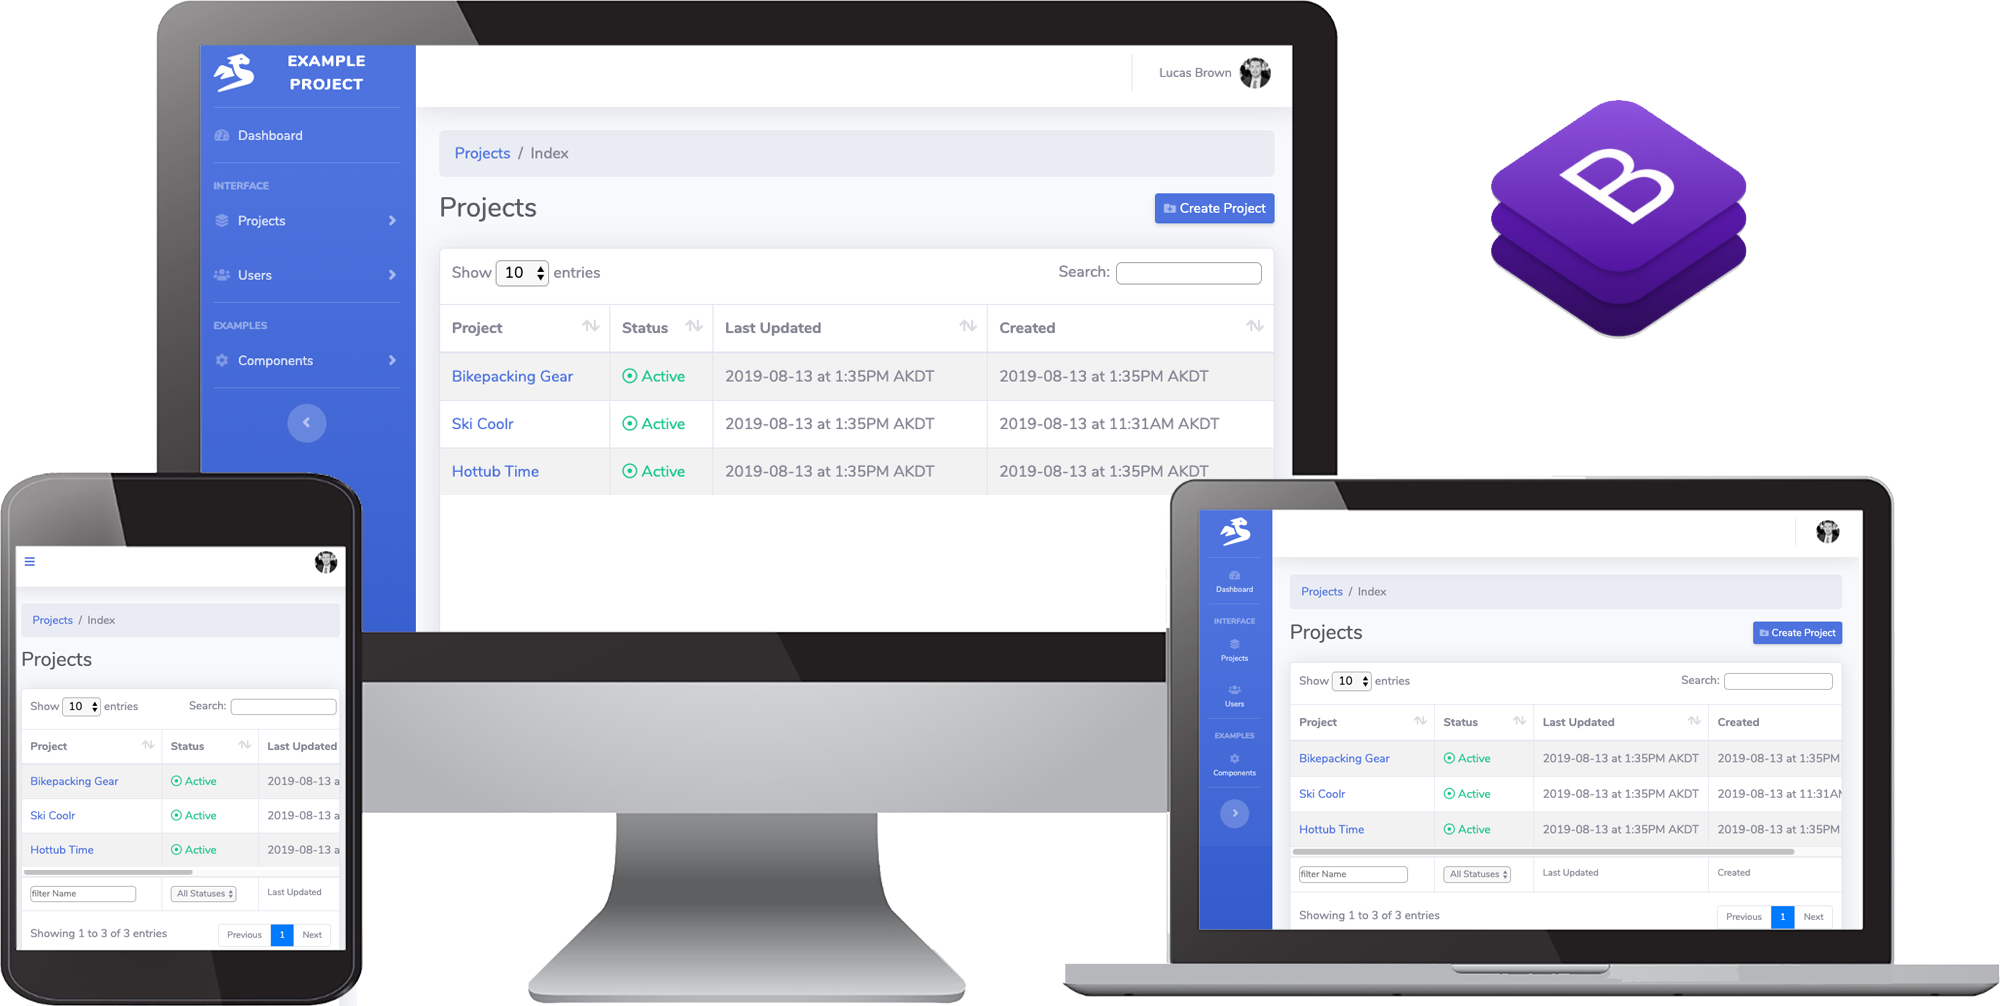
\includegraphics[width=8cm, keepaspectratio]{img/bootstrap.png}
  \caption{Bootstrap.}\label{fig:bootstrap}
\end{figure}


\section{Pandas} 
\label{sec:pandas}

Pandas~\cite{pandas} es una biblioteca construida sobre el lenguaje de programación Python de manipulación y análisis de datos.
Es una herramienta de código abierto, rápida, potente, flexible y fácil de usar.
Proporciona estructuras de datos y herramientas de análisis de datos de alto rendimiento.

\vspace{5mm}
Dispone de tres estructuras de datos diferentes:
\begin{itemize}
    \item \textbf{Series: } estructura de una dimensión cuyos elementos tienen que ser del mismo tipo.
    \item \textbf{DataFrame: } estructura de dos dimensiones en formato ancho o largo (tablas).
    Contiene dos índices (cada uno puede ser de un tipo), uno para las filas y otro para las columnas, y se puede acceder a sus elementos mediante los índices o los nombres de las filas y las columnas.
    \item \textbf{Panel: } estructura de tres dimensiones (cubos).
\end{itemize}

\vspace{5mm}
Algunas características importantes de la herramienta:
\begin{itemize}
    \item Lectura y escritura de datos (CSV, Excel, SQL, JSON, Parquet\ldots).
    \item Inserción y eliminación de columnas en estructuras de datos.
    \item Reestructuración y segmentación de conjuntos de datos, y manejo integrado de los datos faltantes.
    \item Facilita el manejo de series temporales: generación de rangos de fechas y conversión de frecuencias, desplazamiento de ventanas estadísticas y de regresiones lineales, desplazamiento de fechas…
    \item Hace más amigable el uso de NumPy (software de análisis numérico).
\end{itemize}

\section{Visual Studio Code} 
\label{sec:visual-studio-code}

Visual Studio Code~\cite{visualstudio} es un editor de código fuente ligero pero potente que se ejecuta en el escritorio y está disponible para Windows, macOS y Linux.
Se basa en Electron, un framework que se utiliza para implementar Chromium y Node.js como aplicaciones para escritorio.

\vspace{5mm}
Es gratuito, de código abierto y permite ajustar su instalación a las tecnologías de desarrollo que le interese al usuario.
Posibilita la descarga y gestión de extensiones con las que podemos personalizar y potenciar esta herramienta, como lenguajes, depuradores y complementos.
Incluye personalización de atajos de teclado, tema del editor y la configuración de preferencias.

\vspace{5mm}
Viene con soporte incorporado para JavaScript, TypeScript y Node.js, pero gracias a las extensiones también agrega soporte para otros lenguajes como C ++, C\#, Java, Python, etc.

\vspace{5mm}
Además, contiene soporte para la depuración, resaltado de sintaxis, recomendaciones de autocompletado de código, refactorización de código y control integrado de Git.

\begin{figure}[ht]
  \centering
  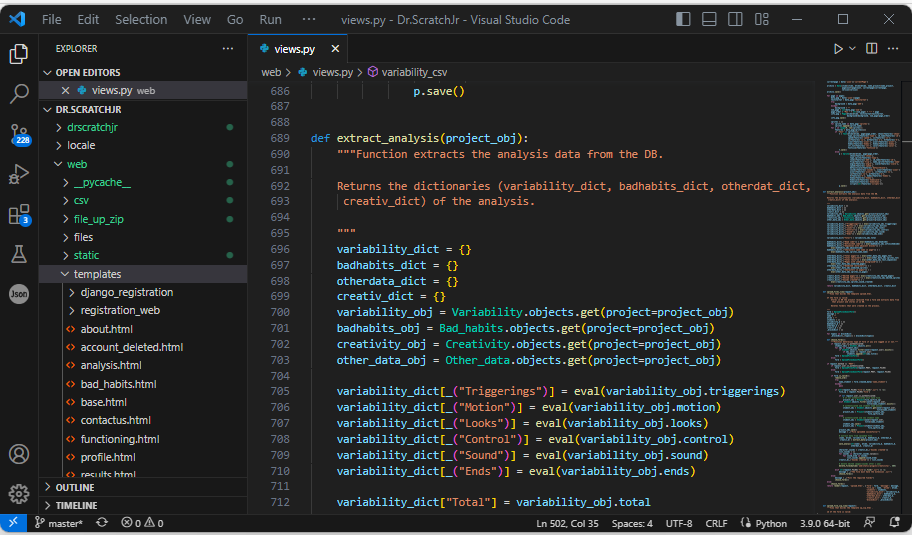
\includegraphics[width=16cm, keepaspectratio]{img/visualstudiocode.png}
  \caption{Visual Studio Code.}\label{fig:visualstudiocode}
\end{figure}


%%%%%%%%%%%%%%%%%%%%%%%%%%%%%%%%%%%%%%%%%%%%%%%%%%%%%%%%%%%%%%%%%%%%%%%%%%%%%%%%
%%%%%%%%%%%%%%%%%%%%%%%%%%%%%%%%%%%%%%%%%%%%%%%%%%%%%%%%%%%%%%%%%%%%%%%%%%%%%%%%
% DISEÑO E IMPLEMENTACIÓN %
%%%%%%%%%%%%%%%%%%%%%%%%%%%%%%%%%%%%%%%%%%%%%%%%%%%%%%%%%%%%%%%%%%%%%%%%%%%%%%%%

\cleardoublepage
\chapter{Diseño e implementación}
\label{chap:implementacion}

En este capítulo se describe la arquitectura y cómo se ha diseñado la aplicación Dr.ScratchJr.

\section{Arquitectura general} 
\label{sec:arquitectura}

\begin{figure}[h!]
  \centering
  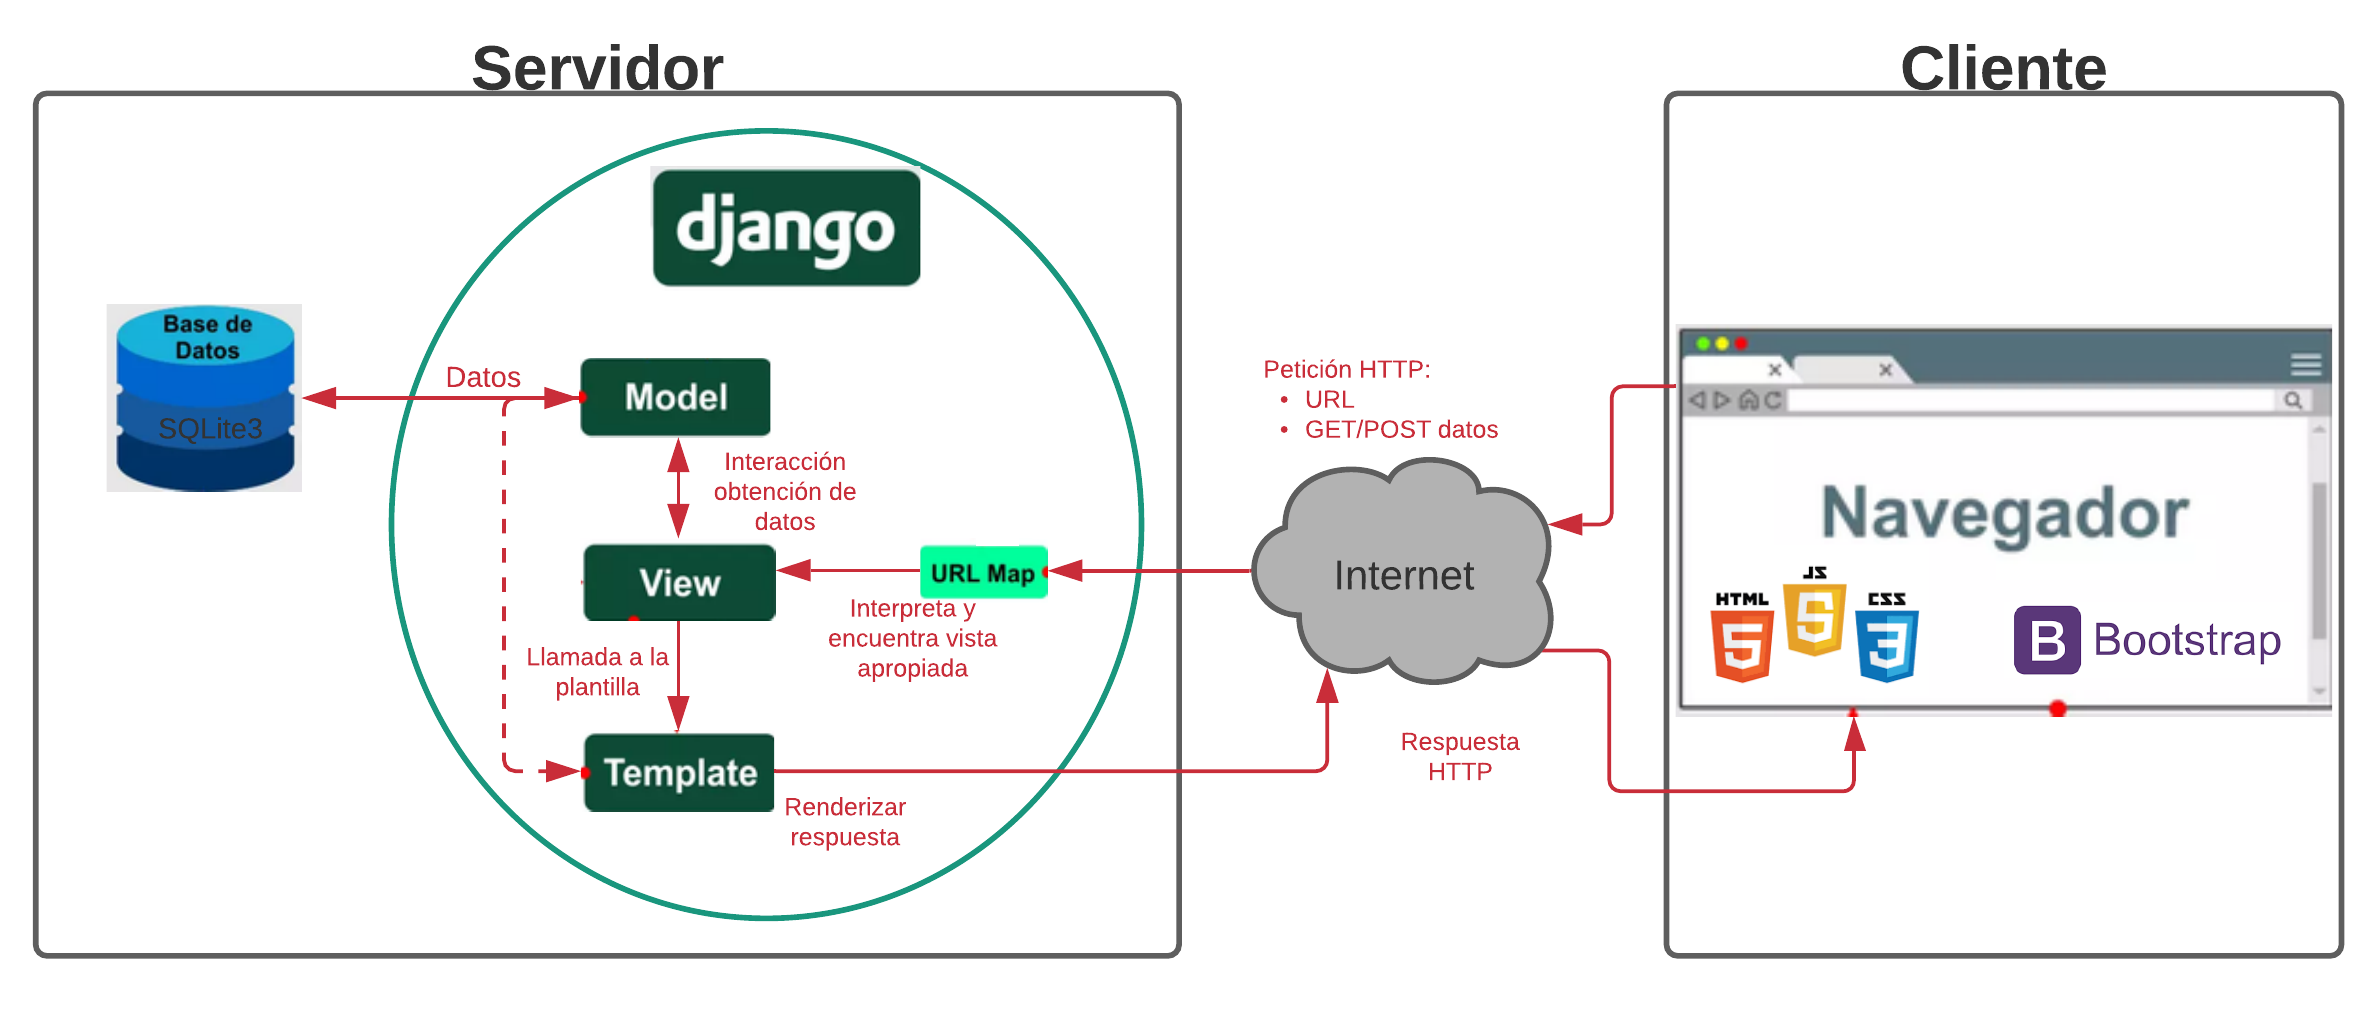
\includegraphics[width=16cm, keepaspectratio]{img/arquitectura.png}
  \caption{Arquitectura de Dr.ScratchJr.}\label{fig:arquitectura}
\end{figure}

La arquitectura que sigue Dr.ScratchJr es la del modelo cliente-servidor.
El usuario a través del navegador web se conecta a la aplicación web Dr.ScrtachJr.
Subirá uno o varios proyectos mediante los formularios que dispone. 
El navegador manda una petición HTTP con una URL que es interpretada por el mapa de URLS (URLmap o URLconf) para encontrar la vista apropiada.
La vista (\emph{View}) valida los datos de los formularios, estructura esos datos e interactúa con el modelo para almacenar y obtener datos.
El modelo (\emph{Model}) define la estructura y Django se encarga de comunicarse con la base de datos.
La plantilla (\emph{Template}) recibe los datos de la vista y luego los organiza para la presentación al navegador a través de una respuesta HTTP.

\section{Algoritmo aplicación} 
\label{sec:algoritmo}

% Algoritmo: Archivos

\vspace{5mm}
El algoritmo que se ha llevado a cabo para la realización de la función principal de la aplicación Dr.ScratchJr, que es analizar proyectos, comienza con la extracción de los datos.
ScratchJr tiene la opción de compartir proyectos vía correo electrónico o AirDrop, lo que genera un archivo con extensión .sjr.
De este archivo SJR es de donde partimos.
Siendo este un archivo comprimido Zip que puede contener carpetas y archivos de recursos dependiendo de los elementos que se usen en la aplicación ScracthJr:

\begin{itemize}
    \item Una carpeta \emph{backgrounds} que contiene imágenes SVG de los fondos de páginas que han sido editados/creados con el editor de ScratchJr.
    No se genera si no se ha usado el editor en el proyecto.
    \item Una carpeta \emph{characters} que contiene imágenes SVG de los personajes (objetos) que han sido editados/creados con el editor de ScratchJr.
    Tampoco se genera si no se ha usado el editor.
    \item Una carpeta \emph{sounds} que contiene los archivos de audio WAV de los personajes (objetos) que han sido creados con el grabador de ScratchJr.
    No se genera si no se han producido grabaciones.
    \item La carpeta \emph{thumbnails} contiene una imágen PNG con la vista de la página que está situada en última posición en un proyecto ScratchJr.
    \item Un fichero \emph{data} que es un archivo JSON con todos los datos del proyecto. Un ejemplo de su jerarquía de datos se muestra en la figura~\ref{fig:jerarquia_json}.
\end{itemize}

\begin{figure}[ht]
  \centering
  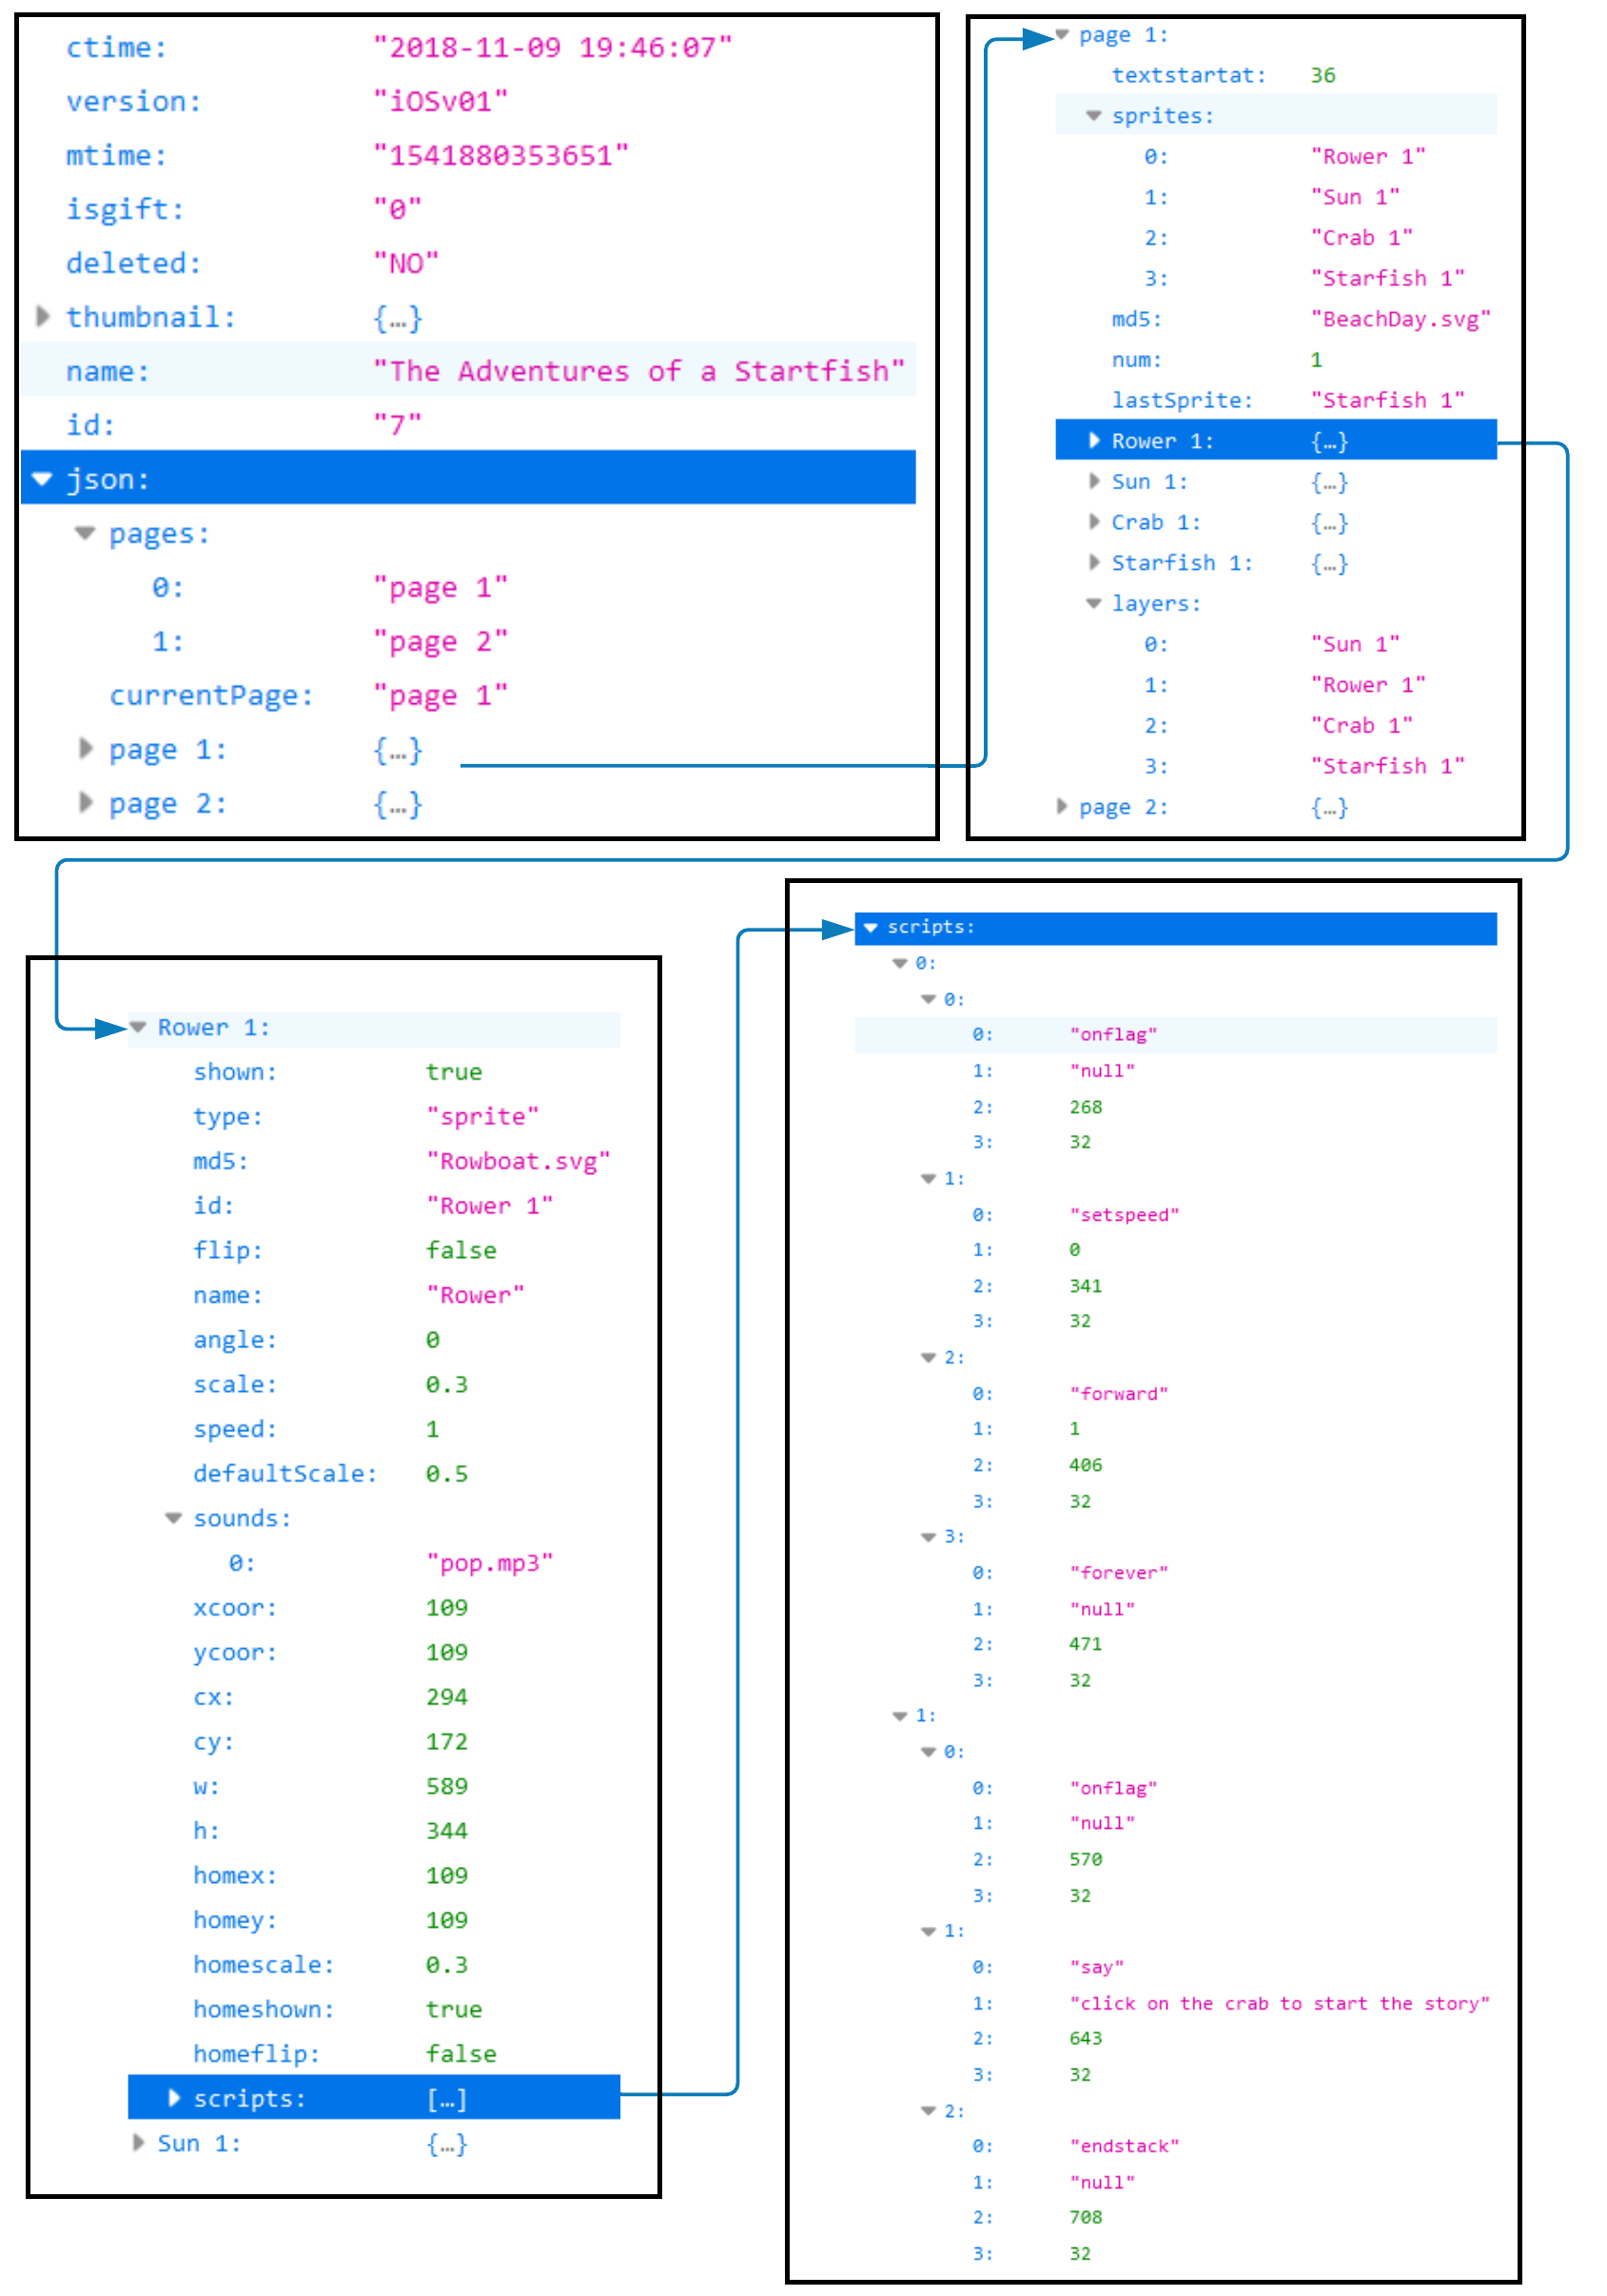
\includegraphics[width=15cm, keepaspectratio]{img/jerarquia_json.png}
  \caption{Ejemplo fichero data.json.}\label{fig:jerarquia_json}
\end{figure}

\clearpage

% Algoritmo: procedimiento
\subsection{Procedimiento}
\label{subsec:procedimiento}
\vspace{5mm}
El procedimiento que se ha seguido para obtener los datos necesarios ha sido:

\begin{itemize}
    \item Descomprimir el archivo zip.
    \item Copiar el contenido de las carpetas \emph{characters}, \emph{backgrounds} y \emph{sounds} en local.
    \item Obtener del archivo \emph{data.json} todos los valores que pueden llegar a ser de utilidad en futuros tipos de análisis de proyectos y almacenarlos en la base de datos (figura~\ref{fig:bd_json}).
    \item Adaptar dichos datos para realizar las distintas variedades del análisis.
\end{itemize}

\begin{figure}[H]
  \centering
  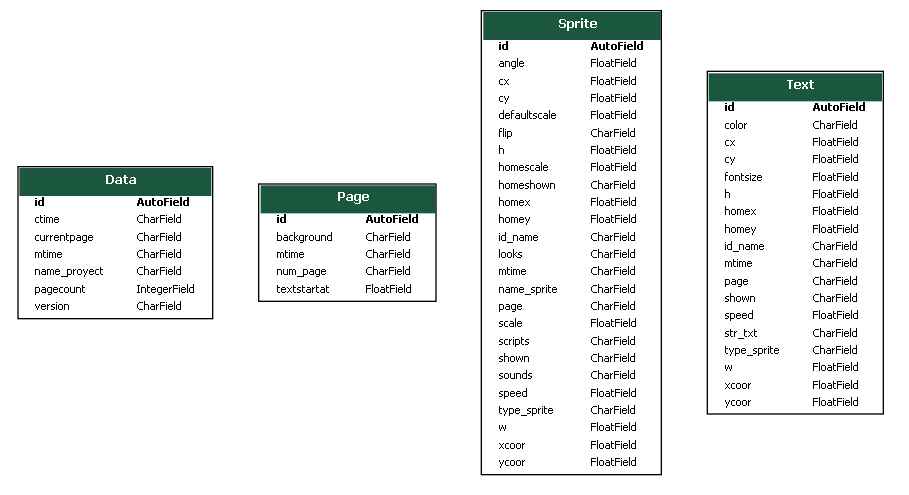
\includegraphics[width=16cm, keepaspectratio]{img/bd_json.png}
  \caption{Datos de la estructura JSON en la base de datos.}\label{fig:bd_json}
\end{figure}

\newpage
% Algoritmo: Criterios
\subsection{Criterios}
\label{subsec:Criterios}

\vspace{5mm}
Para realizar dicho análisis se han llevado a cabo los siguientes criterios: Variabilidad, Creatividad, Malos hábitos y Otros datos.

\begin{itemize}
    \item En el aspecto \emph{Variabilidad} se ha querido evaluar el uso de bloques en el proyecto, es decir la cantidad de bloques distintos que se han utilizado.
    Para ello se distinguen, como en la aplicación ScratchJr, cinco tipos de bloques: Eventos (figura~\ref{fig:evento}), Movimiento (figura~\ref{fig:movimiento}), Apariencia (figura~\ref{fig:apariencia}), Sonido (figura~\ref{fig:sonido}), Control (figura~\ref{fig:control}) y Finalización (figura~\ref{fig:finalizacion}).
    El algoritmo devuelve, para cada uno de los tipos, los bloques que se han empleado al menos una vez en todo el proyecto.

\vspace{5mm}
    En Dr.ScratchJr se ha tomado como la misma clase de bloque, como se puede observar en las figuras~\ref{fig:movimiento} y~\ref{fig:apariencia},  aquéllos que hacen la misma función pero de manera opuesta.
    Como es el caso de los bloques \emph{Girar a la derecha} y \emph{Girar a la izquierda}, \emph{Mover a la derecha} y \emph{Mover a la izquierda}, \emph{Subir} y \emph{Bajar}, \emph{Crecer} y \emph{Disminuir}, y \emph{Mostrar} y \emph{Ocultar}. 
    
\newpage

    \begin{figure}[H]
     \centering
      \subfloat[Evento]{
       \label{fig:evento}
        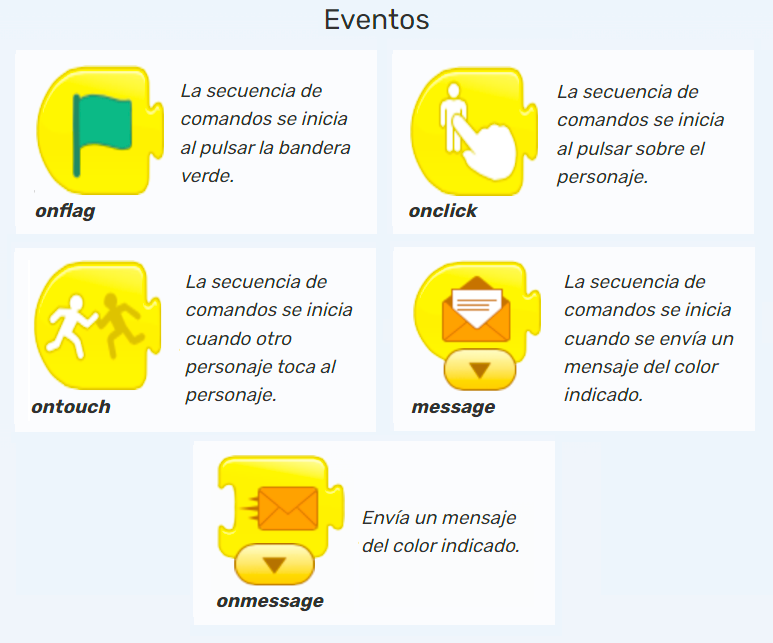
\includegraphics[width=0.49\textwidth]{img/eventos.png}}
      \subfloat[Movimiento]{
       \label{fig:movimiento}
        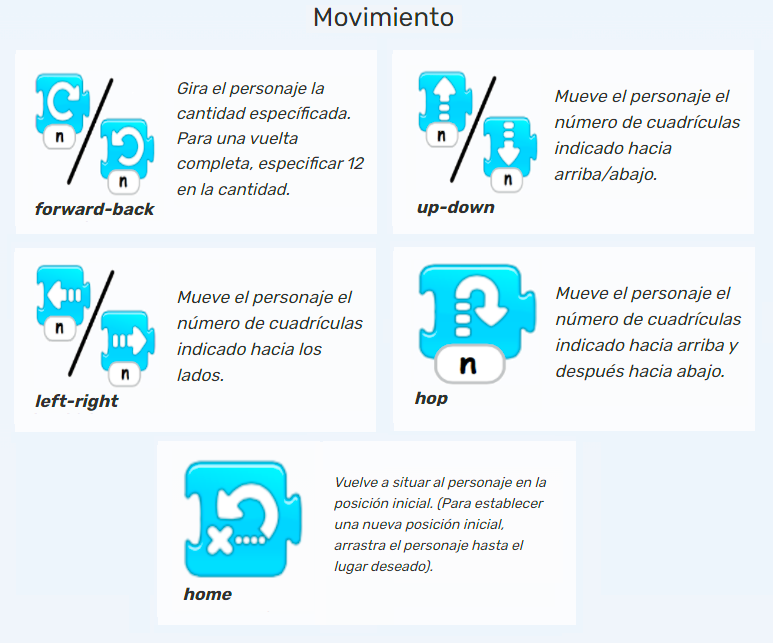
\includegraphics[width=0.49\textwidth]{img/movimiento.png}}
      \vspace{5mm}
      \subfloat[Apariencia]{
       \label{fig:apariencia}
        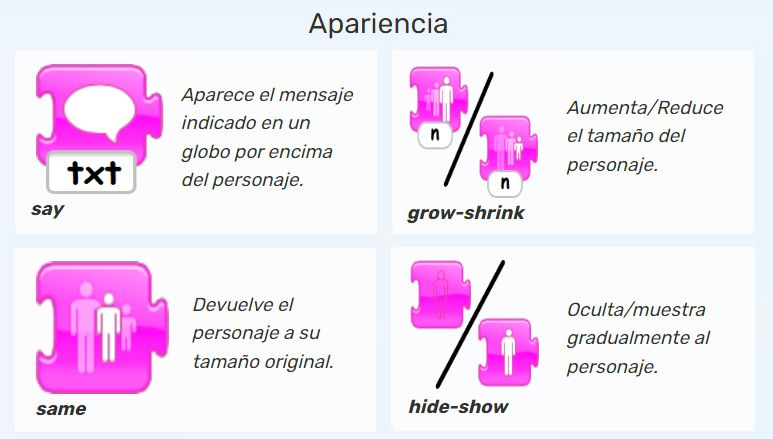
\includegraphics[width=0.49\textwidth]{img/apariencia.png}}
      \subfloat[Sonido]{
       \label{fig:sonido}
        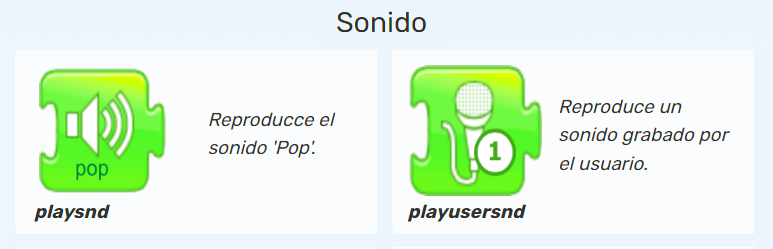
\includegraphics[width=0.49\textwidth]{img/sonido.png}}
     \vspace{5mm}
      \subfloat[Control]{
       \label{fig:control}
        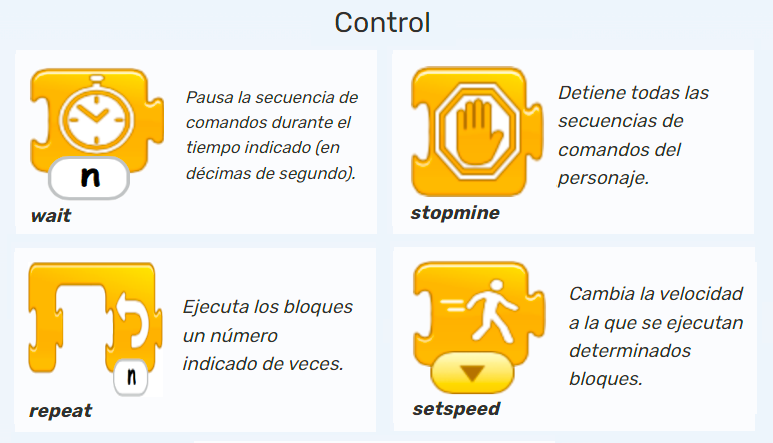
\includegraphics[width=0.49\textwidth]{img/control.png}}
      \subfloat[Finalización]{
       \label{fig:finalizacion}
        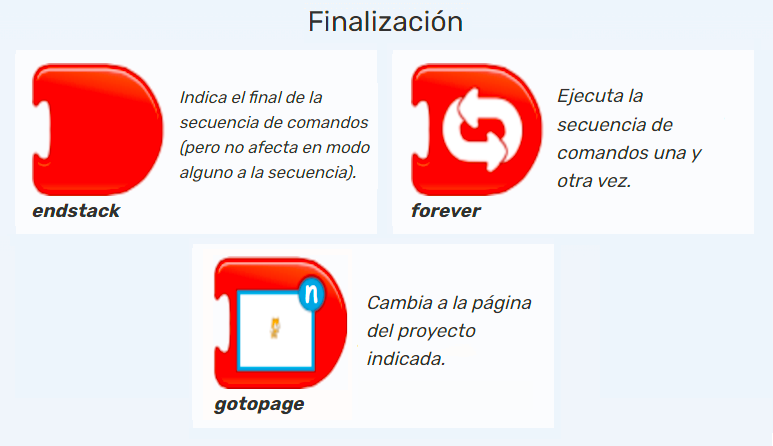
\includegraphics[width=0.49\textwidth]{img/finalizacion.png}}
     \caption{Tipos de bloques en Dr.ScratchJr} \label{fig:bloques}
    \end{figure}
    \newpage
    
    \item Para el criterio \emph{Malos hábitos} se tienen en cuenta algunos errores que se comentan a continuación en las siguientes funciones del código (retornan tanto listas como diccionarios que posteriormente son utilizados para mostrar el análisis completo):
     \begin{itemize}
        \item \emph{dead\_code(adapted\_dict):} función que devuelve una lista con las secuencias de bloques que no comiencen con un bloque de Eventos.
        También están incluidas en la lista las secuencias que comienzan con el bloque ``Comenzar con mensaje'' de un color, pero solo cuando no aparece en el proyecto ningún bloque ``Enviar mensaje'' del mismo color, puesto que esa secuencia nunca se ejecutaría y debe ser considerado código muerto.
        
        \vspace{5mm}
        Para ello, el algoritmo busca el primer bloque de cada secuencia y si no coincide con ninguno de los bloques de Eventos (figura~\ref{fig:evento}), se añade a la lista la secuencia junto con el personaje que la utilice y la página donde se encuentre.
        En el caso de coincidir el primer bloque de una secuencia con el bloque ``Comenzar con mensaje'' de un color, se busca en todas las secuencias de todo el proyecto si existe el bloque ``Enviar mensaje'' de ese mismo color, y si no se encuentra, se añade la secuencia a la lista del mismo modo que se ha comentado antes.

        \item \emph{unfinished\_code(adapted\_dict):} localiza el último bloque de cada secuencia del proyecto y si éste no es un bloque de Finalización (figura~\ref{fig:finalizacion}), añade dicha secuencia, junto con el personaje que la utilice y la página donde se encuentre, a una lista que es devuelta al finalizar la búsqueda en todas las secuencias.

        \item \emph{equal\_adjac\_blocks(adapted\_dict):} busca secuencias con bloques repetidos unidos que puedan ser reemplazados por un solo bloque con atributos.
        Los bloques con atributos son aquellos que se puede indicar el número de veces que se quiere que el personaje haga la acción que indican dichos bloques.
        Por ejemplo, un personaje que utiliza el bloque Subir con atributo 3, hace que dicho personaje se desplace tres cuadriculas hacia arriba.
        
        La función también busca las secuencias que se encuentran dentro de un bloque ``Repetir''. 
        Si encuentra en algún caso bloques repetidos unidos añade la secuencia entera a una lista que es devuelta al acabar la búsqueda.
        
        \item \emph{sprites\_same\_name:} el algoritmo busca si en una página hay más de un personaje con el mismo nombre y si es así, se añade el número de ocasiones que se repite el nombre del personaje como valor en un diccionario cuya clave es el nombre de personaje en concreto.
        Este diccionario, a su vez, se añade como valor de otro diccionario (``sprites\_same\_name'') y con clave la página en la que se encuentran los personajes del mismo nombre.
         \begin{center}
            Ej: \{`Pos 1-page 1': \{`Bat': `3 ocasiones'\}\}.
         \end{center}
     \end{itemize}

    \item Para el criterio \emph{Creatividad} se busca si el usuario ha generado nuevo contenido respecto al contenido que proporciona la aplicación ScratchJr.

    \vspace{5mm}
    El propio programa de ScratchJr aplica el algoritmo MD5 a sus archivos multimedia que tiene por defecto para saber si han sido modificadas.
    Los archivos que han sido modificados por el usuario son nombrados con 32 dígitos hexadecimales.
    Entonces el algoritmo de Dr.ScratchJr considera imágenes editadas o grabaciones de audio, aquellos cuyos archivos tienen un nombre con una longitud mayor a 30 caracteres.
    Estos datos modificados se almacenan en los siguientes diccionarios.
     \begin{itemize}
        \item \emph{edited\_pages:} (páginas editadas) es un diccionario en el que se almacenan como claves las páginas que tienen una imagen de fondo editada y como valores los nombres de las imágenes de fondo.
        \item \emph{edited\_sprites:} (personajes editados) es un diccionario en el que se almacenan como claves los personajes que han sido editados y como valores los nombres de las imágenes de los personajes editados.
        \item \emph{sprites\_sound\_created:} (personajes con grabaciones) es un diccionario en el que se almacenan como claves los personajes que tienen alguna grabación de audio creada y como valor de cada clave una lista con los nombres de todos las grabaciones de audio del personaje.
     \end{itemize}
    
    \item En el apartado \emph{Otros datos} se señalan los siguientes parámetros:
     \begin{itemize}
        \item \emph{sprites\_tot:} lista con los nombres de todos los personajes. Los nombres de los personajes tienen esta estructura:
         \begin{center}
            `` `\textbf{nombre del personaje}' (`\textbf{nombre identificador del texto}') ''
         \end{center}

        \item \emph{pages\_tot:} lista con los nombres de todas las páginas.
        Los nombres de las páginas tienen esta estructura:
         \begin{center}
            ``Pos \textbf{n1} - page \textbf{n2} ''
         \end{center}
        Siendo `n1' el número que corresponde a la posición que tiene la página en Scratch cuando fue guardado el proyecto y `n2' el número que corresponde al orden en el que fue creada esa página por el usuario en ScratchJr.

        \item \emph{unedited\_sprites:} lista con todos los personajes que no han sido editados.
        Estos son almacenados con los nombres de igual forma que la estructurada en la lista ``sprites\_tot''.

        \item \emph{unedited\_pages:} lista de todas las páginas que no han sido editadas, dichas páginas guardadas con el nombre de igual manera que se hacía en la lista ``pages\_tot''.

        \item \emph{sprites\_in\_pages:} diccionario que tiene como claves los nombres de todas las páginas, y como valor de cada clave una lista con el nombre de los personajes que aparecen en esa página.

        \item \emph{text\_sequences:} lista que tiene como elementos tantas listas como textos haya en el proyecto.
        Cada lista tiene la siguiente estructura:
         \begin{center}
            `` [`Pos \textbf{n1} - page \textbf{n2} ', `\textbf{nombre identificador del texto}', [`str\_txt', `\textbf{cadena del texto}'], [`fontsize', `\textbf{tamaño de fuente}']] ''.
         \end{center}
     \end{itemize}
\end{itemize}

\newpage

\begin{figure}[H]
  \centering
  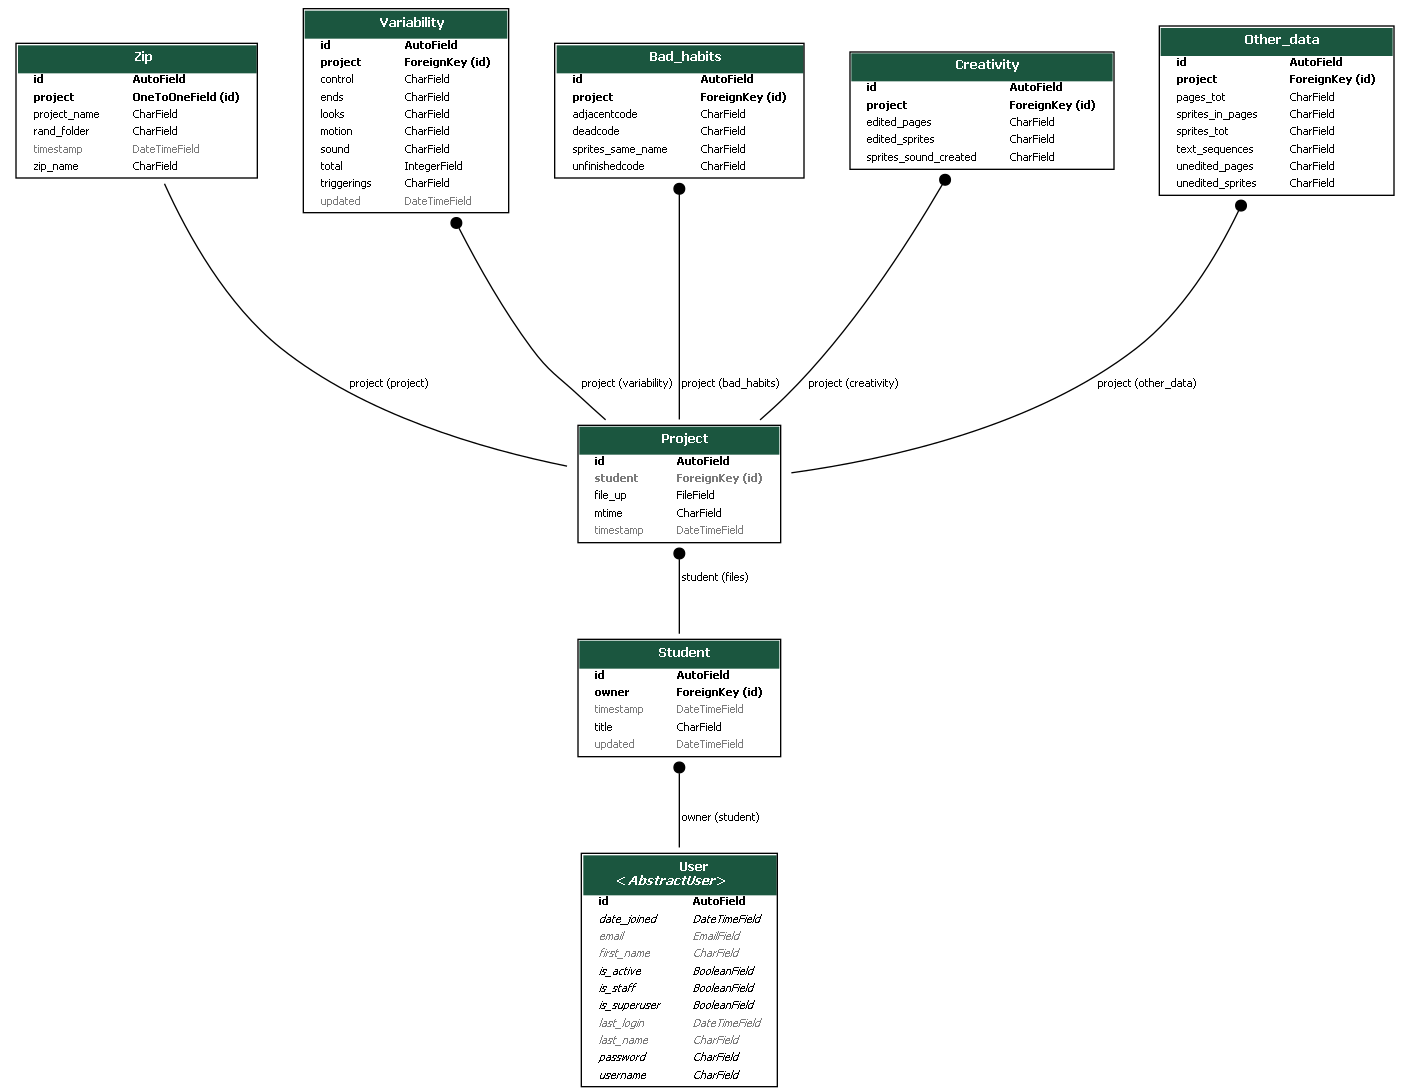
\includegraphics[width=16cm, keepaspectratio]{img/entidad-relacion.png}
  \caption{Esquema entidad-relación de los criterios del análisis.}\label{fig:bd_criterios}
\end{figure}

% Algoritmo: proceso final

Una vez el algoritmo ha abstraído los datos para su análisis, se almacenan y se introducen en diccionarios que se utilizan como contexto para representar (renderizar) las plantillas que muestran los resultados del análisis.
Estos diccionarios se almacenan igualmente en base de datos (figura~\ref{fig:bd_analisis}) de manera temporal para posteriormente utilizarlos también para renderizar las plantillas que muestran los detalles de un tipo de análisis en concreto.

\newpage
\begin{figure}[H]
  \centering
  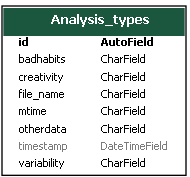
\includegraphics[keepaspectratio]{img/bd_analisis.png}
  \caption{Tabla análisis en la base de datos.}\label{fig:bd_analisis}
\end{figure}

El proceso para el análisis de múltiples proyectos es el mismo salvo que en lugar de representarse primero la plantilla del análisis de un proyecto, se renderiza una plantilla con un listado de los proyectos subidos junto al estudiante asociado a ese proyecto (figura~\ref{fig:listado_zip}).
A partir de ese listado se puede ver el análisis de cada proyecto individualmente.

\vspace{4mm}
\begin{figure}[H]
  \centering
  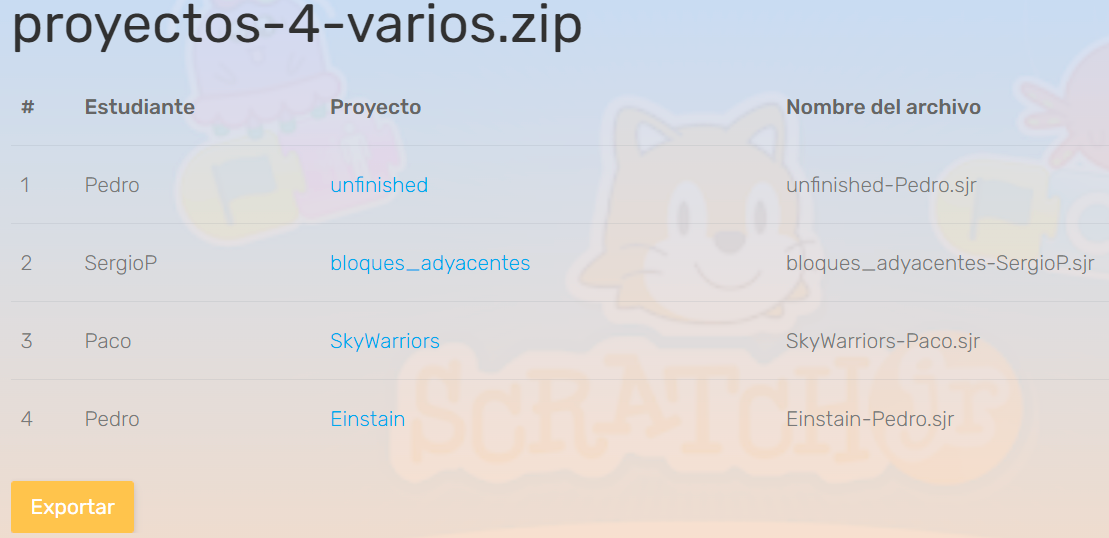
\includegraphics[width=13cm, keepaspectratio]{img/listado_zip.png}
  \caption{Ejemplo de un listado del análisis de un zip.}\label{fig:listado_zip}
\end{figure}

En cualquier listado con proyectos en la aplicación web Dr.ScratchJr existe la posibilidad de exportar los datos del análisis de los proyectos. 
Al exportar se genera un zip, los datos se almacenan en tres ficheros CSV (badhabits-1, otherdata-1, variability-1) y en una hoja de cálculo de Microsoft Excel llamada data.xlsx con los mismos datos de los tres ficheros CSV, pero agrupados en pestañas en un solo documento.

\vspace{5mm}
Dr.ScratchJr dispone de la opción de cambiar a su pagina web el idioma a español o a inglés gracias al módulo gettext, disponible en Django, y creando los archivos de traducción para cada uno de los lenguajes.

\section{Página web}
\label{sec:pagina-web}

Al acceder a la aplicación web sin estar identificado desde un ordenador se muestran dos cuadros donde el usuario puede introducir uno o varios proyectos a la vez para que sean analizados, una breve presentación donde sugiere que el usuario se registre para poder almacenar los análisis que suba a la herramienta y un panel lateral en el lado izquierdo para ayudar al usuario.

El primer cuadro sirve para cargar un proyecto de ScratchJr, con extensión .sjr, a fin de visualizar su análisis al instante.
En el caso de que se esté registrado en Dr.ScratchJr aparecerá también un recuadro donde podrás asociar dicho proyecto con su autor, si este ya existe, o crear uno nuevo, y poder almacenar su análisis para posteriores visualizaciones.

El segundo cuadro da la posibilidad de cargar varios proyectos de una sola vez.
Para ello, es necesario haber almacenado previamente los proyectos con extensión .sjr en un archivo comprimido .zip. Y es este archivo comprimido el que hay que cargar en este cuadro.
Los archivos deben de ser nombrados con la estructura ``\textbf{`Nombre del proyecto'}-\textbf{`Nombre del estudiante'}.sjr'' para poder ser almacenados correctamente y poder asociarlos a sus autores.
Al cargar el zip y pinchar en analizar se muestra una página con un listado de los proyectos que contiene el zip con la opción de modificar el nombre con el que se desea guardar el proyecto en la aplicación.
En el caso de haber iniciado sesión, también existe la opción de cambiarle el nombre al estudiante en cada proyecto (figura~\ref{fig:pag_subida_zip}).

\begin{figure}[H]
     \centering
      \subfloat[Sin loguear]{
       \label{fig:subir_zip}
        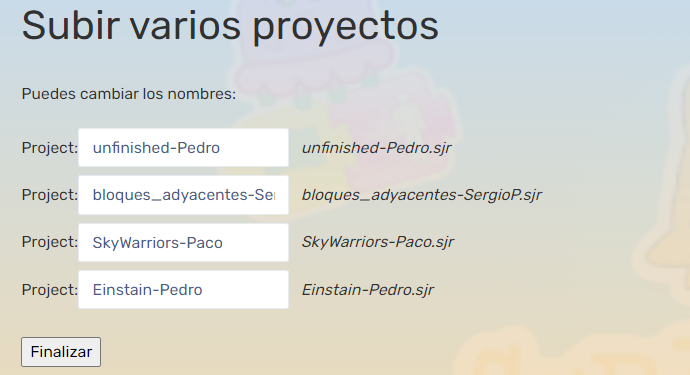
\includegraphics[width=0.49\textwidth]{img/subir_zip_.png}}
      \subfloat[Logueado]{
       \label{fig:subir_zip_logueado}
        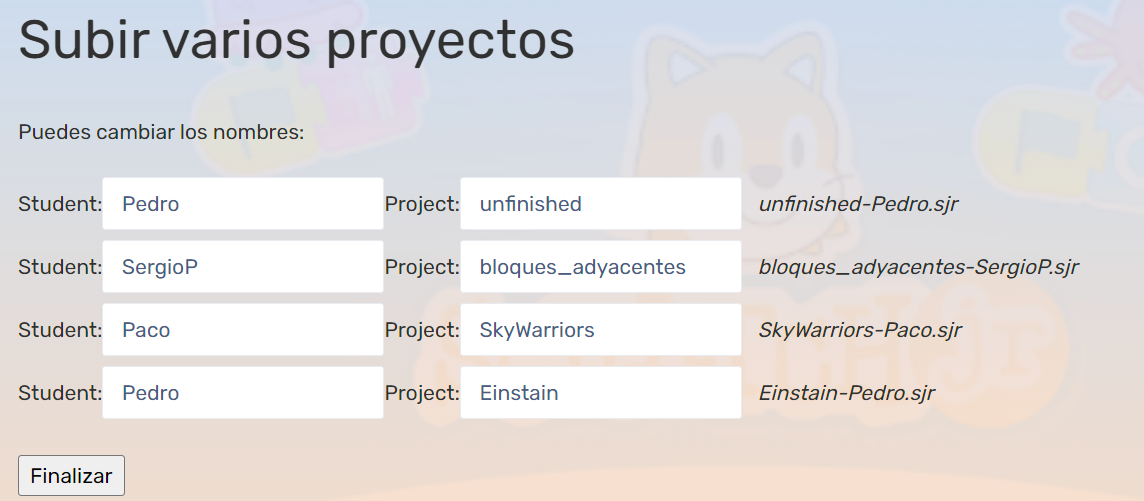
\includegraphics[width=0.49\textwidth]{img/subir_zip_logueado.png}}
     \caption{Página tras subir un zip de proyectos.} \label{fig:pag_subida_zip}
\end{figure}
% 

\newpage
\subsection{Direcciones URLs de la aplicación}
\label{subsec:Tabla de urls con sus vistas}

    \begin{table}[H]
     La tabla~\ref{tabla:path-url} hace un breve resumen de la funcionalidad de las vistas que están asociadas a las URLs de la aplicación web Dr.ScratchJr.
     \begin{center}
     \begin{tabular}{ | m{3.1cm} | m{3.3cm} | m{8.8cm} | }
      \hline \textbf{Path URL} & \textbf{Vista} & \textbf{Función}\\ \hline
    
        `` '' &
        home\_view &
        Página principal de la aplicación con formularios para cargar proyectos \\ \hline
        
        profile/ &
        profile\_view &
        Información sobre el usuario registrado y el número de estudiantes que tiene almacenados. Permite modificar algunos datos del usuario \\ \hline 
        
        settings/ &
        settings\_view &
        Opciones para cambiar o restablecer contraseña, eliminar cuenta o cerrar sesión \\ \hline
        
        functioning/ &
        functioning\_view &
        Información sobre el manejo por Dr.ScratchJr \\ \hline
        
        contactus/ &
        contactus\_view &
        Formulario para contactar con responsables de Dr.ScratchJr \\ \hline
        
        about/ &
        about\_view &
        Información como correo y enlace a Github de Dr.ScratchJr \\ \hline
        
        variability/ &
        variability\_view &
        Información sobre el criterio Variabilidad \\ \hline
        
        bad\_habits/ &
        bad\_habits\_view &
        Información sobre el criterio Malos hábitos \\ \hline
        
        create\_csv\_zip/ \newline $<$str:zip\_name$>$/ \newline $<$str:rand\_folder$>$/ &
        create\_csv\_zip &
        Vista que no renderiza ninguna página, sino que crea un fichero CSV con los datos de los proyectos de un zip \\ \hline
        
        create\_csv\_student/ \newline $<$str:student$>$/ &
        create\_csv\_student &
        Vista que no renderiza ninguna página, sino que crea un fichero CSV con los datos de los proyectos de un estudiante \\ \hline
        
        create\_csv\_user/ &
        create\_csv\_user &
        Vista que no renderiza ninguna página, sino que crea un fichero CSV con los datos de todos los proyectos de todos los estudiantes que tenga almacenado un usuario \\ \hline
        
        albums/upload/ &
        upload\_files\_view &
        Si no se ha cargado ningún proyecto previamente aparecerá un formulario para cargar un proyecto. En el caso de que si, muestra el resultado del análisis \\ \hline 
    
      \end{tabular}
     \end{center}
    \end{table}
    
    \begin{table}[H]
     \begin{center}
      \begin{tabular}{ | m{3.1cm} | m{3.3cm} | m{8.8cm} | }
        \hline \textbf{Path URL} & \textbf{Vista} & \textbf{Función}\\ \hline
    
        albums/upload\_zip/ &
        upload\_file\_zip\_view &
        Si no se ha cargado ningún archivo zip previamente con proyectos aparecerá un formulario para cargar un zip.
        En el caso de que se acabe de subir el zip, muestra un listado de los proyectos con opción a renombrarlos.
        Y una vez finalizado muestra una tabla con los proyectos que contiene el zip con opción de ver cada análisis individualmente \\ \hline 
        
        analysis/ \newline $<$student$>$/ \newline $<$name\_file$>$/ &
        analysis\_view &
        Análisis del proyecto perteneciente a un estudiante \\ \hline
        
        analysis2/ \newline $<$student$>$/ \newline $<$project$>$/ \newline $<$file\_name$>$/ \newline $<$rand\_folder$>$/ &
        analysis2\_view &
        Muestra el análisis de un proyecto individualmente cuando se accede desde el listado de proyectos al cargar un zip \\ \hline 
        
        results/ \newline $<$file\_name$>$/ \newline $<$mtime$>$/ \newline $<$type1$>$/ \newline $<$type2$>$/ &
        results\_view &
        Muestra con más detalles el resultado de un criterio del análisis \\ \hline 
        
        review/ &
        review\_view &
        Tabla de los estudiantes que están almacenados por el usuario, junto con el número de proyectos de cada uno. Opciones de editar el nombre, eliminar estudiantes y exportar todos los proyectos \\ \hline
        
        students/ \newline $<$str:student$>$/ &
        student\_view &
        Tabla con los proyectos de un estudiante en concreto. 
        Opciones de editar el nombre, eliminar proyectos y exportar todos los proyectos \\ \hline
        
        delete/ \newline $<$str:student$>$/ \newline $<$str:file\_name$>$/ \newline $<$str:times$>$/ & 
        delete\_regist &
        Misma tabla que en ``student\_view'', pero sin el proyecto eliminado \\ \hline
    
      \end{tabular}
     \end{center}
    \end{table}
    
    \begin{table}[H]
     \begin{center}
      \begin{tabular}{ | m{3.1cm} | m{3.3cm} | m{8.8cm} | }
        \hline \textbf{Path URL} & \textbf{Vista} & \textbf{Función}\\ \hline
    
        delete\_student/ \newline $<$student$>$/ & 
        delete\_student & 
        Misma tabla que en ``review\_view'', pero sin el estudiante eliminado \\ \hline  
        
        edit\_student/ \newline $<$old\_student$>$/ \newline $<$new\_student$>$/ &
        edit\_student &
        Misma tabla que en ``review\_view'', pero con el nombre del estudiante modificado \\ \hline  
        
        edit\_file/ \newline $<$old\_file$>$/ \newline $<$student$>$/ \newline $<$new\_file$>$/ &
        edit\_file &
        Misma tabla que en ``student\_view'', pero con el nombre del proyecto modificado \\ \hline  
        
        delete\_account/ &
        delete\_account &
        Página de confirmación de cuenta de usuario recién eliminada \\ \hline  
        
        accounts/login/ &
        LoginView &
        Página para iniciar sesión, restablecer contraseña o Registrarse \\ \hline  
        
        accounts/logout/ &
        LogoutView &
        Página de cierre de sesión del usuario \\ \hline  
        
        accounts/ \newline password\_change/ &
        PasswordChange-\newline View &
        Formulario para cambio de contraseña \\ \hline  
        
        accounts/ \newline 
        password\_change/ \newline done/ &
        PasswordChange-\newline DoneView &
        Página de confirmación de contraseña cambiada \\ \hline   
        
        accounts/ \newline password\_reset/ &
        PasswordResetView &
        Formulario donde se introduce el correo de la cuenta para restablecer la contraseña \\ \hline  
        
        accounts/ \newline password\_reset/ \newline done/ &
        PasswordReset- \newline DoneView &
        Página de confirmación de correo correcto para el envío de las instrucciones para restablecer contraseña \\ \hline  
        
        accounts/ \newline reset/done/ &
        PasswordReset-\newline CompleteView &
        Página de confirmación de contraseña restablecida \\ \hline 
    
    
       \end{tabular}
      \caption{Tabla explicativa de las URLs}
      \label{tabla:path-url}
     \end{center}
    \end{table}

\subsection{Vista del análisis}
\label{subsec:Vista del analisis}

La página que muestra el análisis de un proyecto consta de 4 secciones:
\begin{itemize}
    \item Variabilidad (Uso de bloques) (figura~\ref{fig:variabilidad}): esta sección contiene un listado con los tipos de bloques que existen, con unos niveles asociados a cada uno.
    Se distinguen, como en la aplicación ScratchJr, seis tipos de bloques: Eventos (figura~\ref{fig:evento}), Movimiento (figura~\ref{fig:movimiento}), Apariencia (figura~\ref{fig:apariencia}), Sonido (figura~\ref{fig:sonido}), Control (figura~\ref{fig:control}) y Finalización (figura~\ref{fig:finalizacion}).
    El nivel individual es la cantidad de bloques que se han empleado al menos una vez en todo el proyecto sobre los bloques totales que contiene cada tipo. 
    Cabe destacar que Dr.ScratchJr toma como el mismo bloque aquellos que hacen la misma función, pero de manera opuesta, como se puede observar en las figuras~\ref{fig:movimiento} y~\ref{fig:apariencia}.
    Además, esta sección contiene el nivel total, que es la suma de todos los bloques que se han usado al menos una vez sobre la suma del total de bloques de cada tipo.
     \begin{figure}[H]
       \centering
       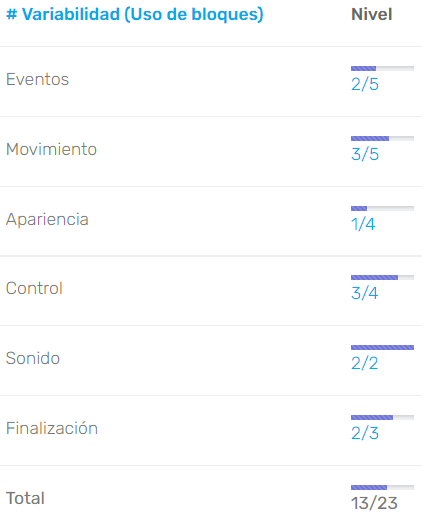
\includegraphics[keepaspectratio]{img/variabilidad.PNG}
       \caption{Sección Variabilidad.}
       \label{fig:variabilidad}
     \end{figure}
    Existe la opción de obtener más detalles pinchando sobre cualquier nivel obtenido de los tipos de bloques, y aparecerá una vista que mostrará aquellos bloques que no han sido usados en el proyecto (figura~\ref{fig:variabilidad-nivel-detalles}).
    \begin{figure}[H]
       \centering
       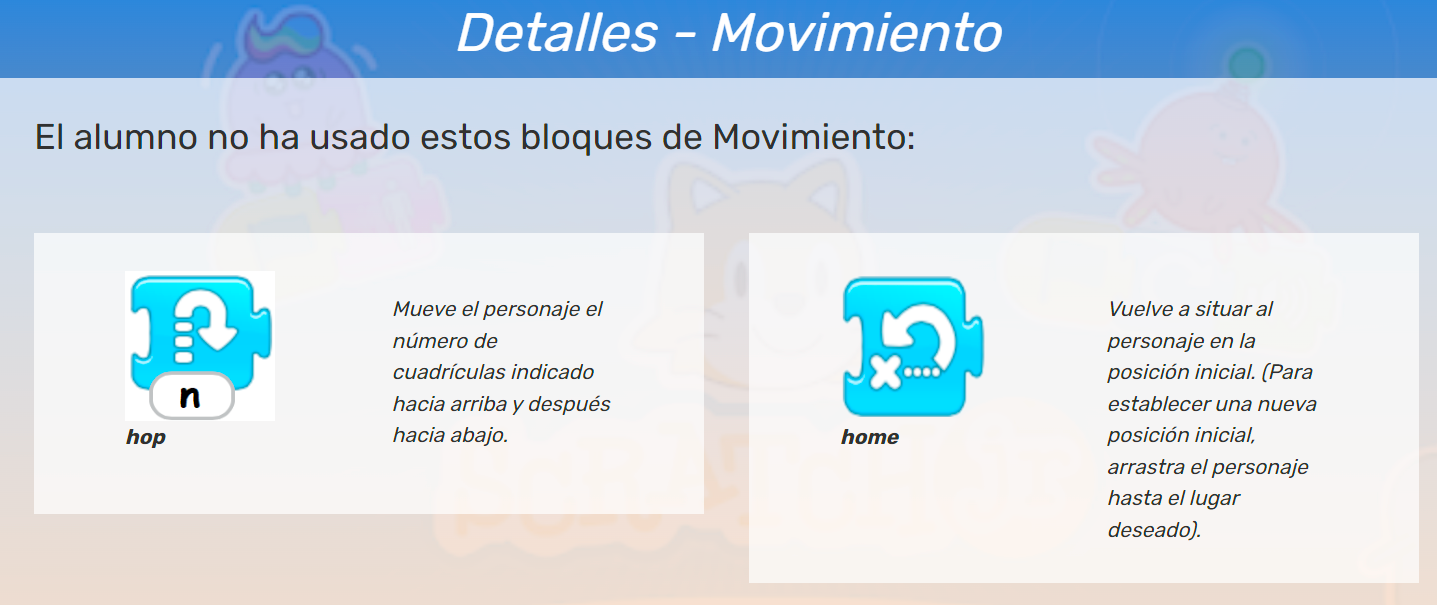
\includegraphics[width=16cm, keepaspectratio]{img/variabilidad-nivel-detalles.PNG}
       \caption{Ejemplo detalles del apartado Movimiento de la sección Variabilidad.}\label{fig:variabilidad-nivel-detalles}
    \end{figure}

    \item Malos hábitos (figura~\ref{fig:malos-habitos}): aquí se muestra la cantidad de ciertos tipos de errores encontrados en el proyecto que el creador debe evitar:
     \begin{itemize}
        \item Código muerto: cantidad de secuencias de bloques que no se van a ejecutar porque no comienzan por un bloque de Evento. 
        También es considerado código muerto cuando una secuencia comienza por el bloque de Evento `Comenzar con mensaje' de un color, pero no hay en el proyecto un bloque `Enviar mensaje' del mismo color.
        
        \item Código inacabado: cantidad de secuencias de bloques que no terminan con un bloque de `Finalización'.
        Estas secuencias se van a ejecutar, pero es conveniente cerrar la secuencia por calidad del código y aprendizaje hacia buenas prácticas de programación.
        
        \item Secuencias con bloques adyacentes: cantidad de secuencias que tienen bloques contiguos iguales.
        Es un mal hábito porque se debe usar un solo bloque e indicar el número de veces que se repite la acción del bloque.

        \item Personajes con mismo nombre en una página: aparece, para cada página donde ocurra esto, el personaje que se repite y el número de ocasiones que lo hace.
        Aunque el personaje se visualice en ScratchJr, se debe nombrar correctamente al crearlo para que no haya varios con el mismo nombre en una única página.
     \end{itemize}    
    \begin{figure}[H]
       \centering
       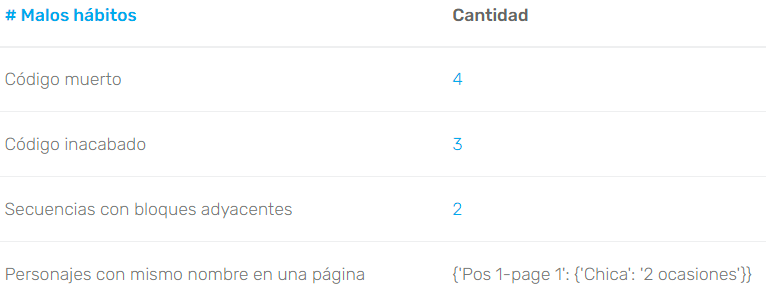
\includegraphics[width=16cm, keepaspectratio]{img/maloshabitos.PNG}
       \caption{Ejemplo de Malos hábitos.}
       \label{fig:malos-habitos}
    \end{figure}
        
    Salvo en este último caso de malos hábitos (personajes con mismo nombre en una página), se encuentra la opción de pinchar en los resultados para obtener más detalles mostrados en forma de tabla con la siguiente estructura: página, personaje, nombre secuencia y secuencia (figura~\ref{fig:bloques-adyac-detalles}). 
    \begin{figure}[H]
        \centering
        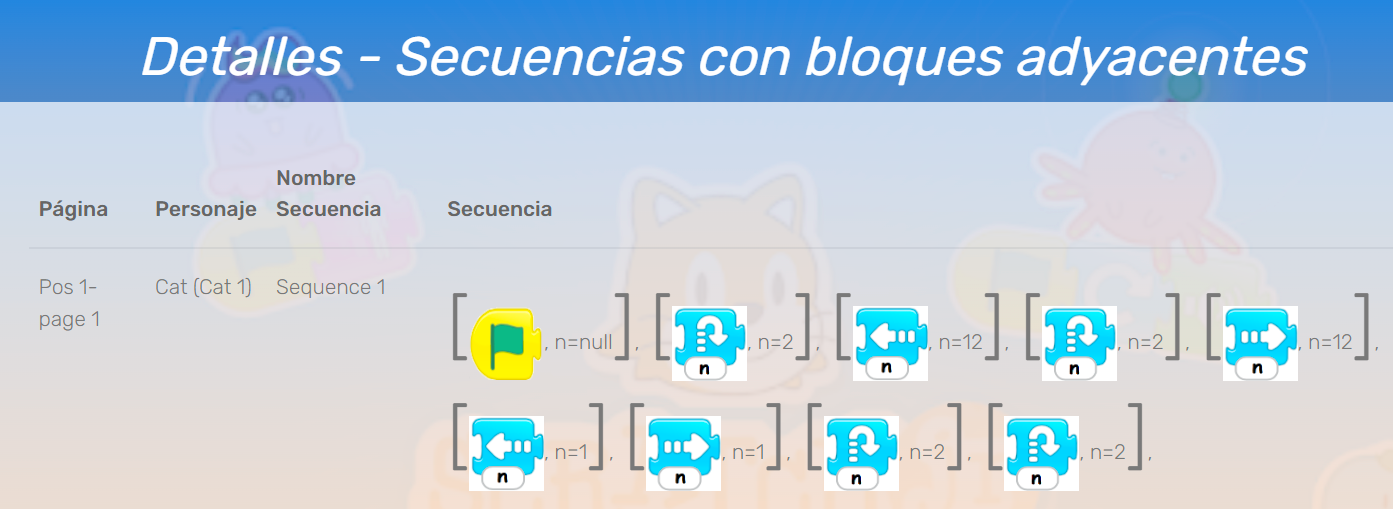
\includegraphics[width=16cm, keepaspectratio]{img/maloshabitos-ady-detalles.PNG}
        \caption{Ejemplo detalles de bloques adyacentes de la sección Malos hábitos.}
        \label{fig:bloques-adyac-detalles}
    \end{figure}

    \item Creatividad (figura~\ref{fig:creatividad}): muestra si el usuario ha generado nuevo contenido para hacer su proyecto en relación a:
     \begin{itemize}
        \item Páginas editadas: cantidad de páginas que tienen su imagen de fondo editada respecto a las imágenes que vienen por defecto, o ha creado un fondo completamente nuevo en una página en blanco con el editor de pintura de ScratchJr.
        \item Personajes editados: número de personajes que han sido editados a través del editor de ScratchJr.
        Con este editor se puede cambiar el nombre del personaje, por lo que al cambiar el nombre también se considera un personaje editado, aunque su apariencia no haya cambiado.
        \item Sonidos creados: cantidad de sonidos que han sido grabados en el proyecto mediante el grabador de ScratchJr.
     \end{itemize}
    \begin{figure}[H]
        \centering
        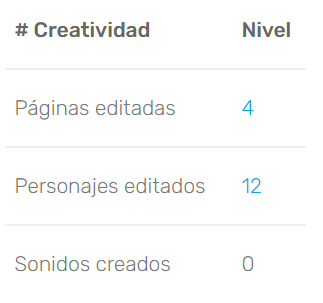
\includegraphics[ keepaspectratio]{img/creatividad.PNG}
        \caption{Ejemplo sección Creatividad.}
        \label{fig:creatividad}
    \end{figure}
    Al pinchar sobre las cantidades de páginas o personajes editados, se puede ver la imagen correspondiente a cada página o personaje editado (figura~\ref{fig:personajes-editados-detalles}).
    Además pinchando en la imagen se puede ver en tamaño completo en una pestaña nueva.
    \begin{figure}[H]
        \centering
        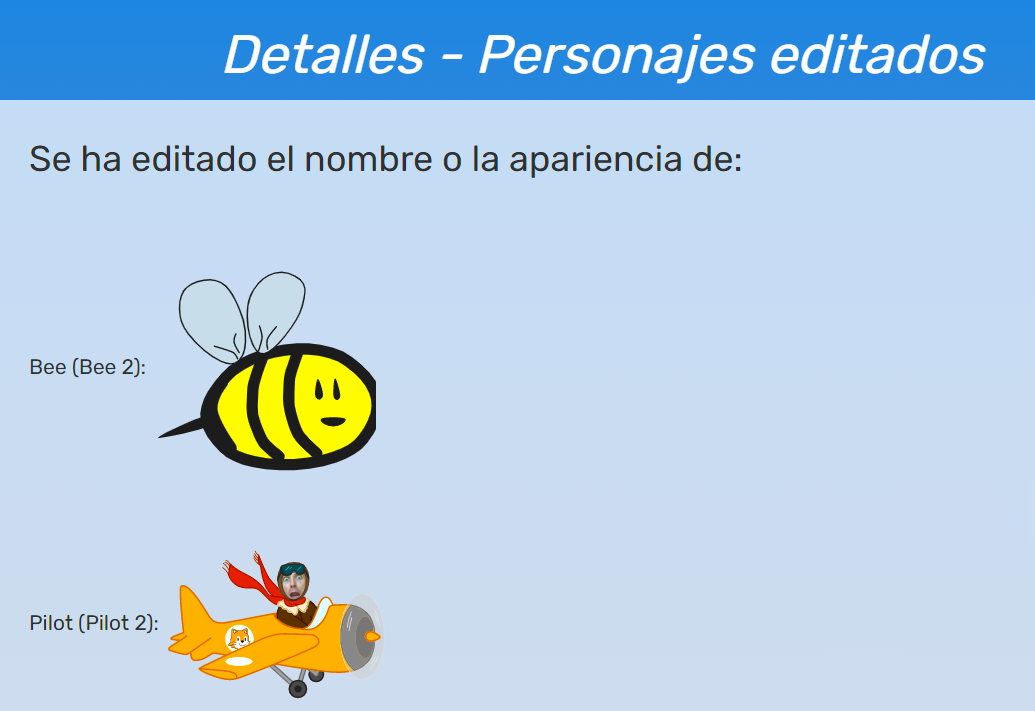
\includegraphics[width=11cm, keepaspectratio]{img/creatividad-detalles-personajes.PNG}
        \caption{Ejemplo detalles de personajes editados de la sección Creatividad.}
        \label{fig:personajes-editados-detalles}
    \end{figure}
    
    \item Otros datos (figura~\ref{fig:otros_datos}): contiene un listado con datos que pueden llegar a ser de interés para analizar un proyecto:
     \begin{itemize}
        \item Total de páginas: número de páginas que se han utilizado para todo el proyecto.
        \item Total de personajes: número total de personajes empleados en todo el proyecto.
        \item Total de textos: cantidad de textos creados en el proyecto.
        \item Páginas con fondo sin editar: número de páginas que han sido utilizadas tal cual están disponibles en la aplicación ScratchJr por defecto.
        \item Personajes sin editar: cantidad de personajes que han sido utilizados sin cambiar su nombre y sin editar su apariencia, respecto a los personajes por defecto que dispone ScratchJr.
        \item Personajes en páginas: aparece, para cada página, los personajes utilizados en cada una de ellas.
     \end{itemize}
    \begin{figure}[H]
        \centering
        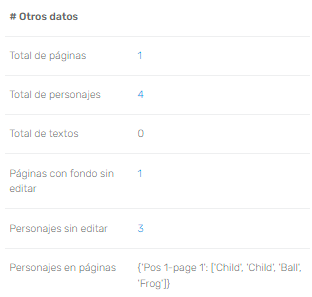
\includegraphics[width=11cm, keepaspectratio]{img/otros_datos.PNG}
        \caption{Ejemplo sección Otros datos.}
        \label{fig:otros_datos}
    \end{figure}
\end{itemize}

\newpage
\subsection{Vista de listados}
\label{subsec:Vista de listados}

\vspace{5mm}
Los tipos de listados que puede haber son:
\begin{itemize}
    \item De un archivo zip: listado mencionado anteriormente (figura~\ref{fig:listado_zip}) de análisis de múltiples proyectos.
    Contiene un listado de los proyectos que están comprimidos en el zip, junto a los estudiantes asociados a dichos proyectos.
    Posibilidad de exportar los datos del análisis de todos los proyectos que contenga el zip.
    \item Estudiantes (figura~\ref{fig:listado_estudiantes}): se accede principalmente desde el panel lateral.
    Muestra todos los estudiantes que tenga el usuario y el número de proyectos de cada estudiante.
    Se encuentra la posibilidad de editar el nombre y/o eliminar a cualquier estudiante junto con todos los proyectos con los que esté asociado.
    En este listado se pueden exportar los datos del análisis de todos los proyectos de todos los estudiantes que tenga el profesor de una sola vez.
    \begin{figure}[H]
      \centering
      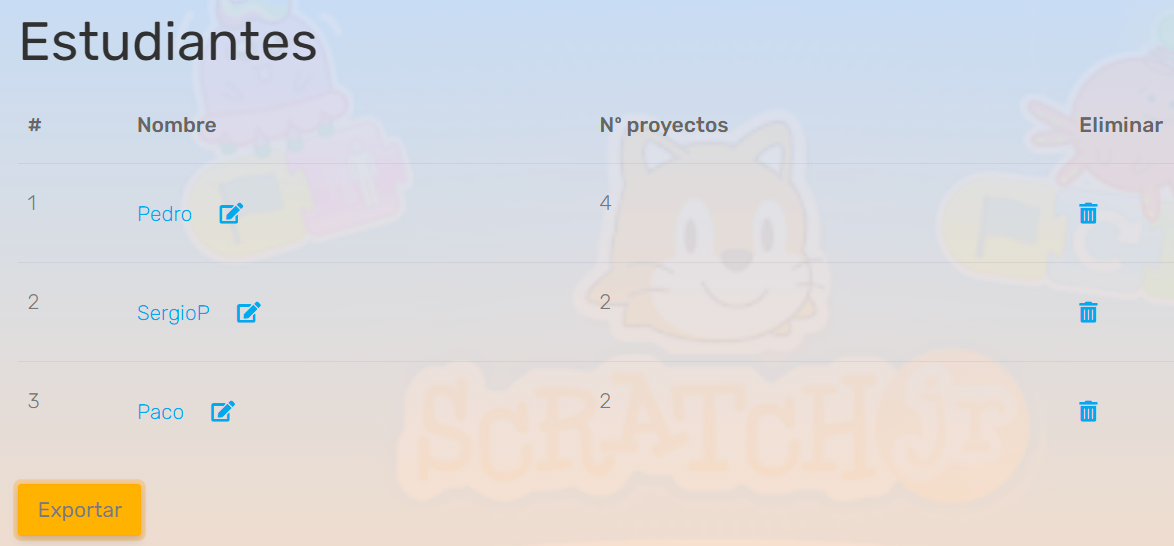
\includegraphics[width=16cm, keepaspectratio]{img/listado_estudiantes.png}
      \caption{Ejemplo de un listado de los estudiantes de un usuario.}\label{fig:listado_estudiantes}
    \end{figure}
    \item Estudiante (figura~\ref{fig:listado_estudiante}): contiene un listado de los proyectos de un estudiante en particular.
    Además de la fecha, una nota del criterio de Variabilidad y el número de Malos hábitos del proyecto.
    También se puede editar el nombre de un proyecto y/o eliminar un proyecto en concreto.
    Posibilidad de exportar los datos del análisis de todos los proyectos del estudiante.
    \begin{figure}[H]
      \centering
      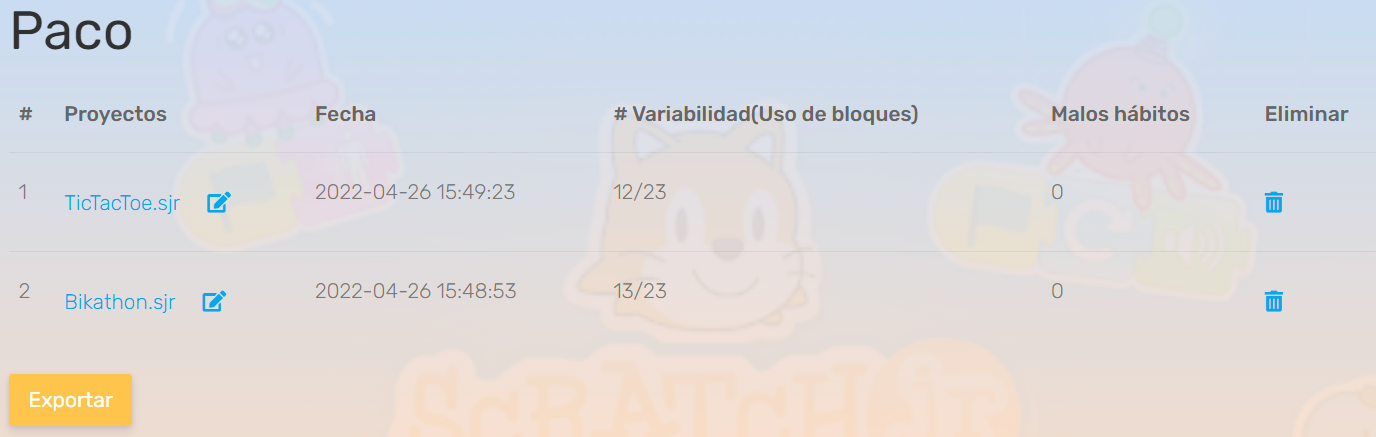
\includegraphics[width=16cm, keepaspectratio]{img/listado_estudiante.png}
      \caption{Ejemplo de un listado de los proyectos de un estudiante de un usuario.}
      \label{fig:listado_estudiante}
    \end{figure}
\end{itemize}
Como ya se ha mencionado, al exportar se genera un zip que contiene tres ficheros CSV (badhabits-1, otherdata-1, variability-1) y una hoja de cálculo (data.xlsx) con los datos del análisis de tantos proyectos como tenga el listado desde donde se haya exportado.


%%%%%%%%%%%%%%%%%%%%%%%%%%%%%%%%%%%%%%%%%%%%%%%%%%%%%%%%%%%%%%%%%%%%%%%%%%%%%%%%
%%%%%%%%%%%%%%%%%%%%%%%%%%%%%%%%%%%%%%%%%%%%%%%%%%%%%%%%%%%%%%%%%%%%%%%%%%%%%%%%
% EXPERIMENTOS Y VALIDACIÓN %
%%%%%%%%%%%%%%%%%%%%%%%%%%%%%%%%%%%%%%%%%%%%%%%%%%%%%%%%%%%%%%%%%%%%%%%%%%%%%%%%

\cleardoublepage
\chapter{Experimentos, validación y resultados}
\label{chap:experimentos}

\section{Ejemplo de un análisis}
\label{sec:Test1_analisis}

Para validar los distintos aspectos del análisis, se ha usado un proyecto de ejemplo llamado Test1.sjr cuyo contenido se presenta en la figura~\ref{fig:Test1}. 
Para ello, seguimos todos los aspectos que incluye un análisis de Dr.ScratchJr y comprobamos que concuerdan los resultados del análisis con los esperados.

\vspace{5mm}
Test1.sjr posee un total de dos páginas, la primera con una imagen de fondo del interior del océano y la segunda con una imagen de una playa.
La primera página contiene los personajes ``Buceador'' y dos ``Caballito de mar'' y la segunda los personajes ``Perro'' y ``Remero'', haciendo un total de 5 personajes en el proyecto. 
Hay un texto ``Playa Blanca'' en la página 2, siendo el único texto del proyecto. 
La primera página con una imagen de fondo del interior del océano no ha sido cambiada por el editor de ScratchJr y es de las que dispone el programa por defecto.
Al igual ocurre con cuatro de los cinco personajes que tiene el proyecto, que son los que proporciona la aplicación y no han sido editados.

\newpage
\begin{figure}[H]
 \centering
  \subfloat[Buceador]{
   \label{fig:buceador}
    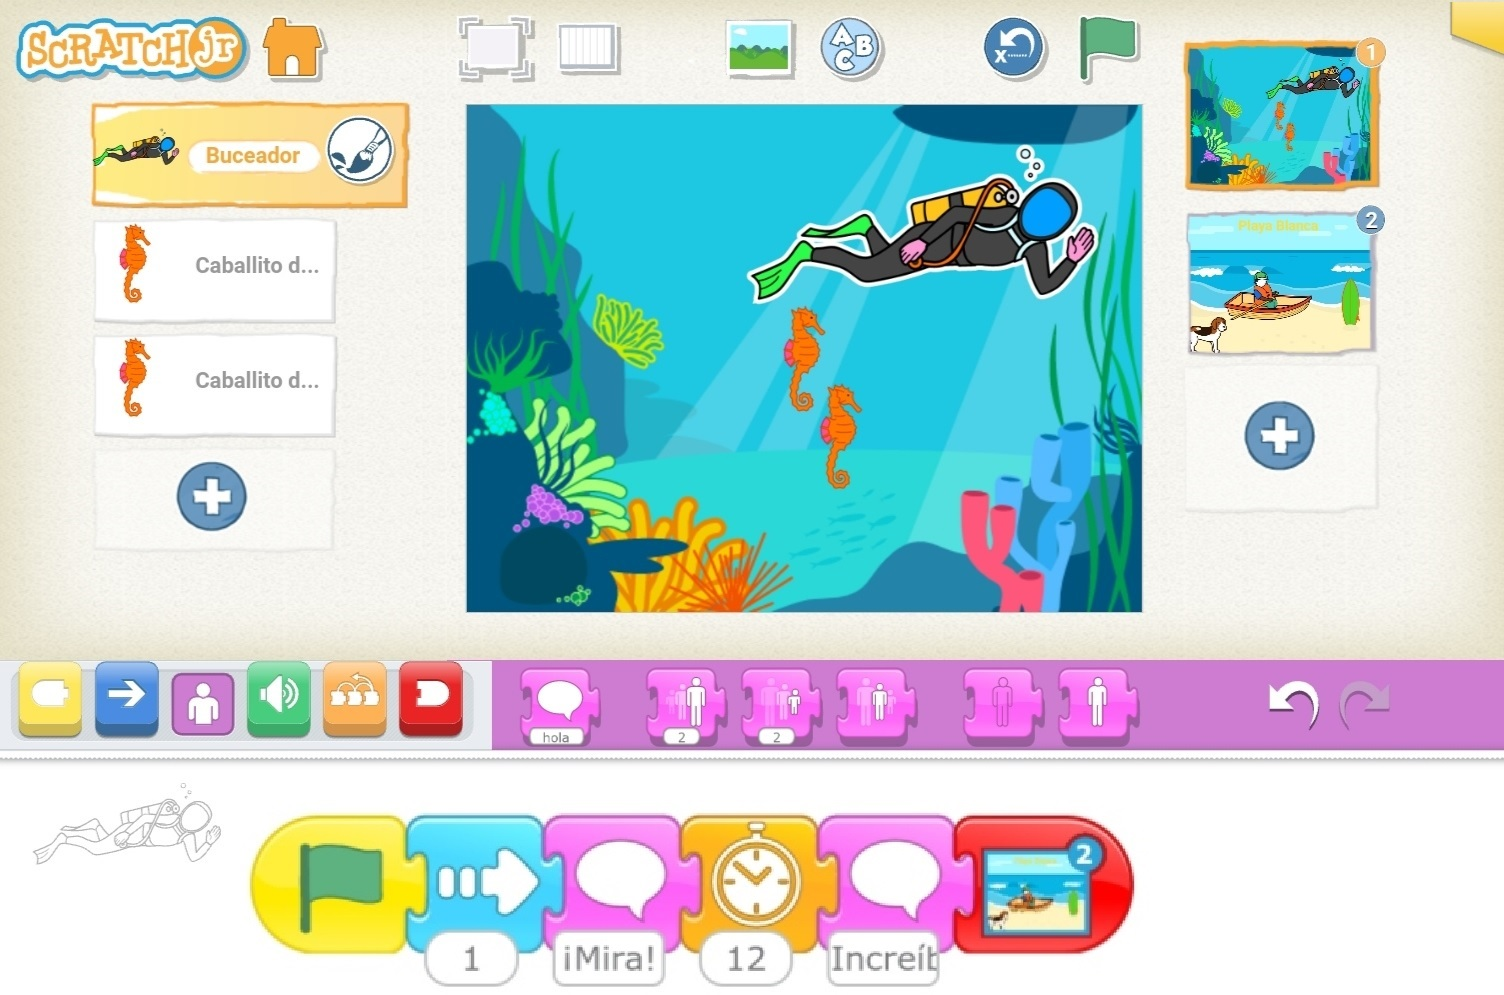
\includegraphics[width=0.50\textwidth]{img/buceador_test.jpg}}
    \hfill
  \subfloat[Caballito 1]{
   \label{fig:caballito1}
    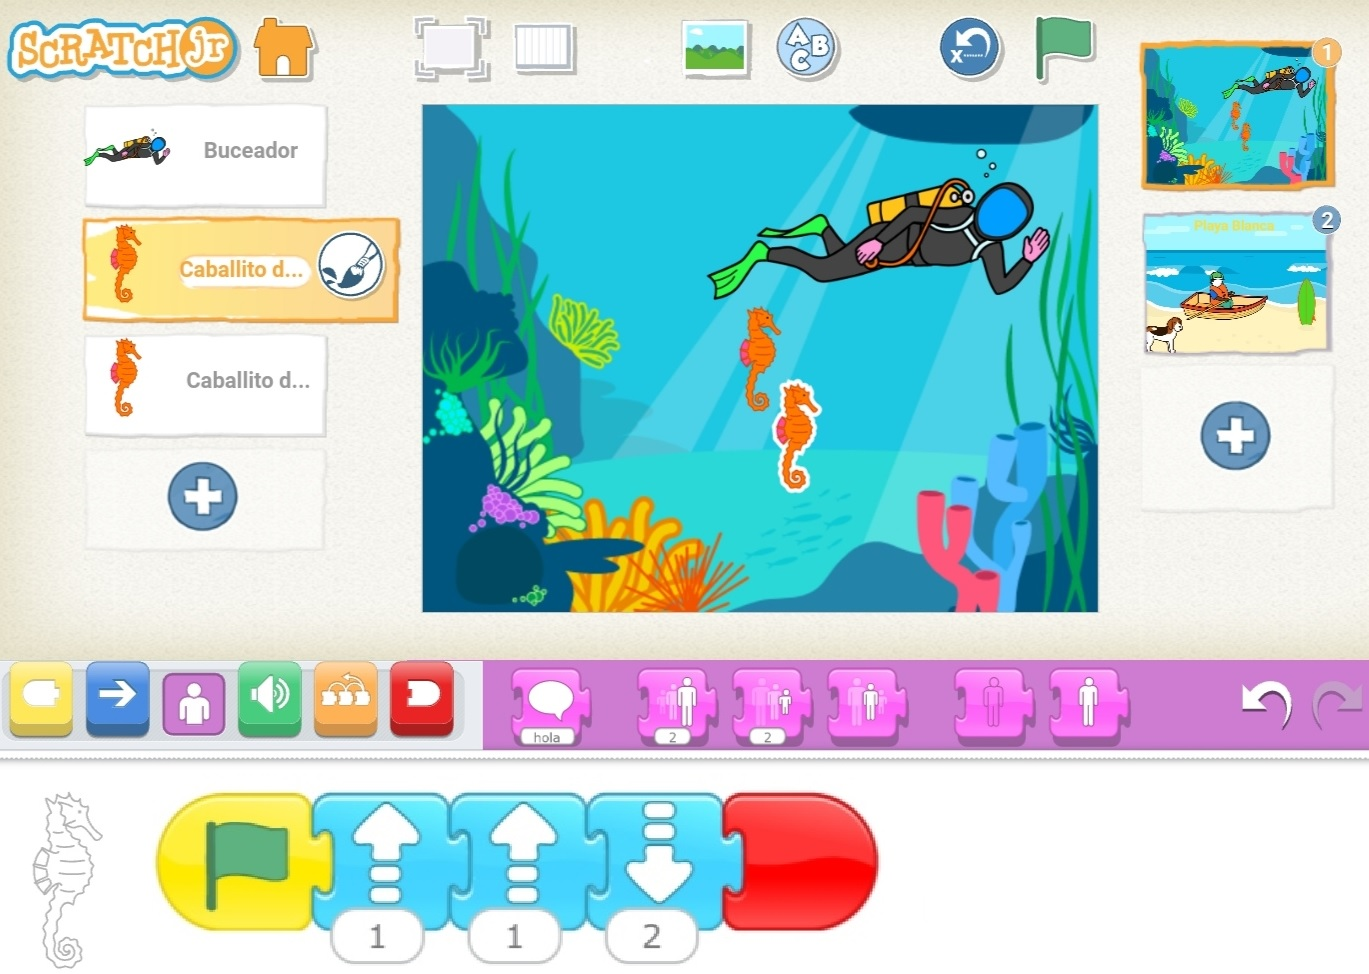
\includegraphics[width=0.47\textwidth]{img/caballito1_test.jpg}}
  \vspace{6mm}
  \subfloat[Caballito 2]{
   \label{fig:caballito2}
    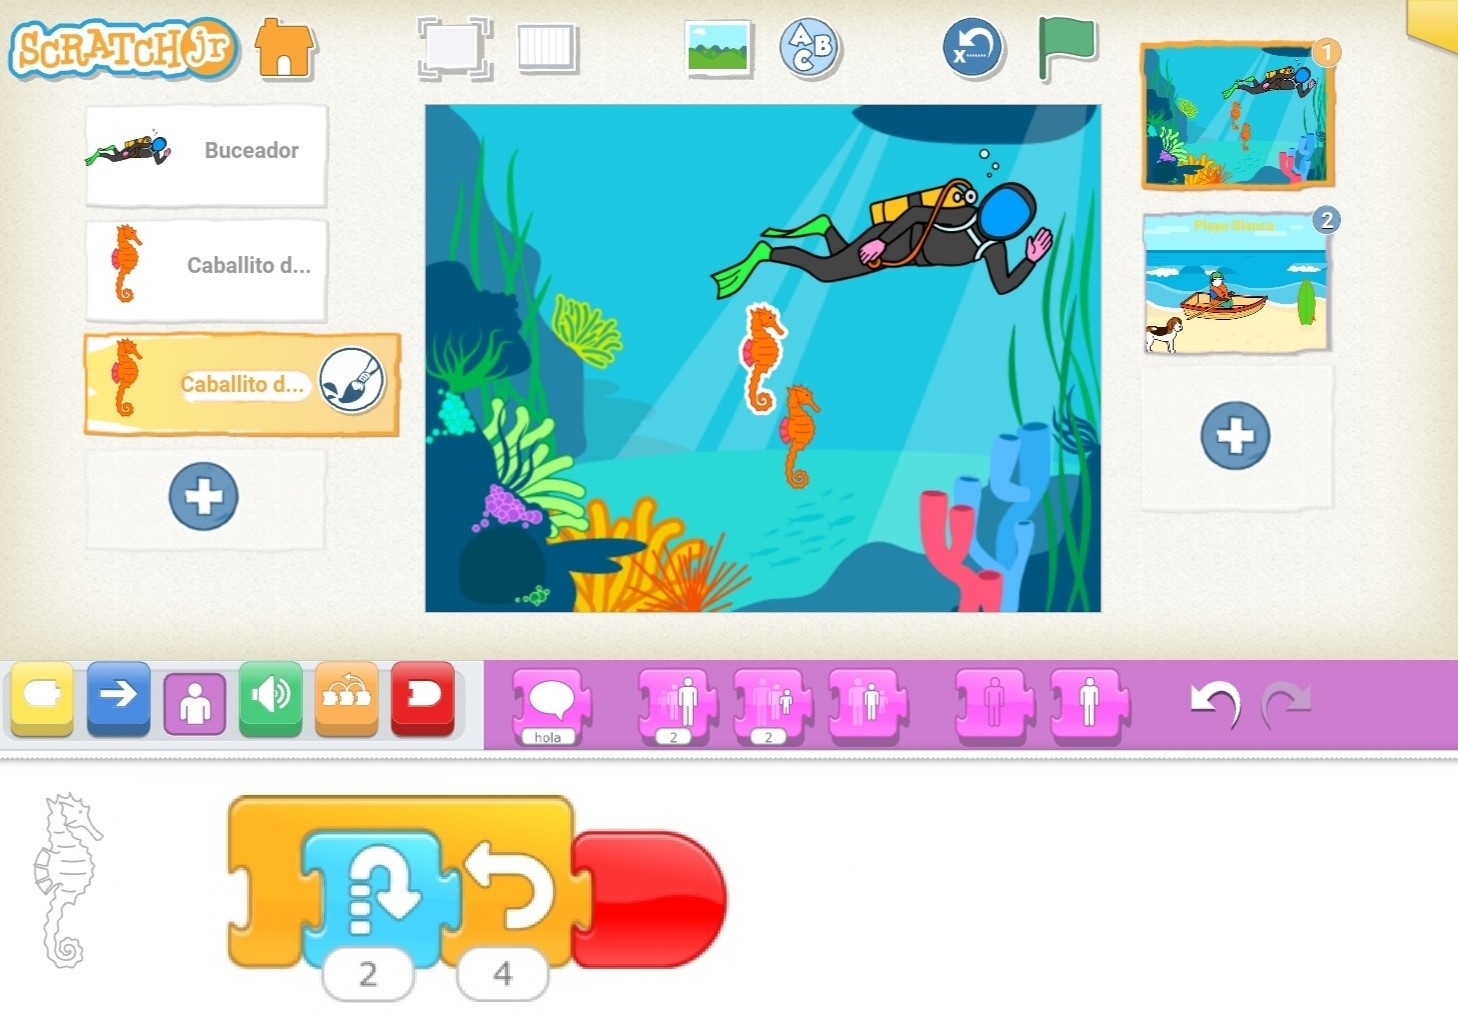
\includegraphics[width=0.48\textwidth]{img/caballito2_test.jpg}}
    \hfill
  \subfloat[Perro]{
   \label{fig:perro}
    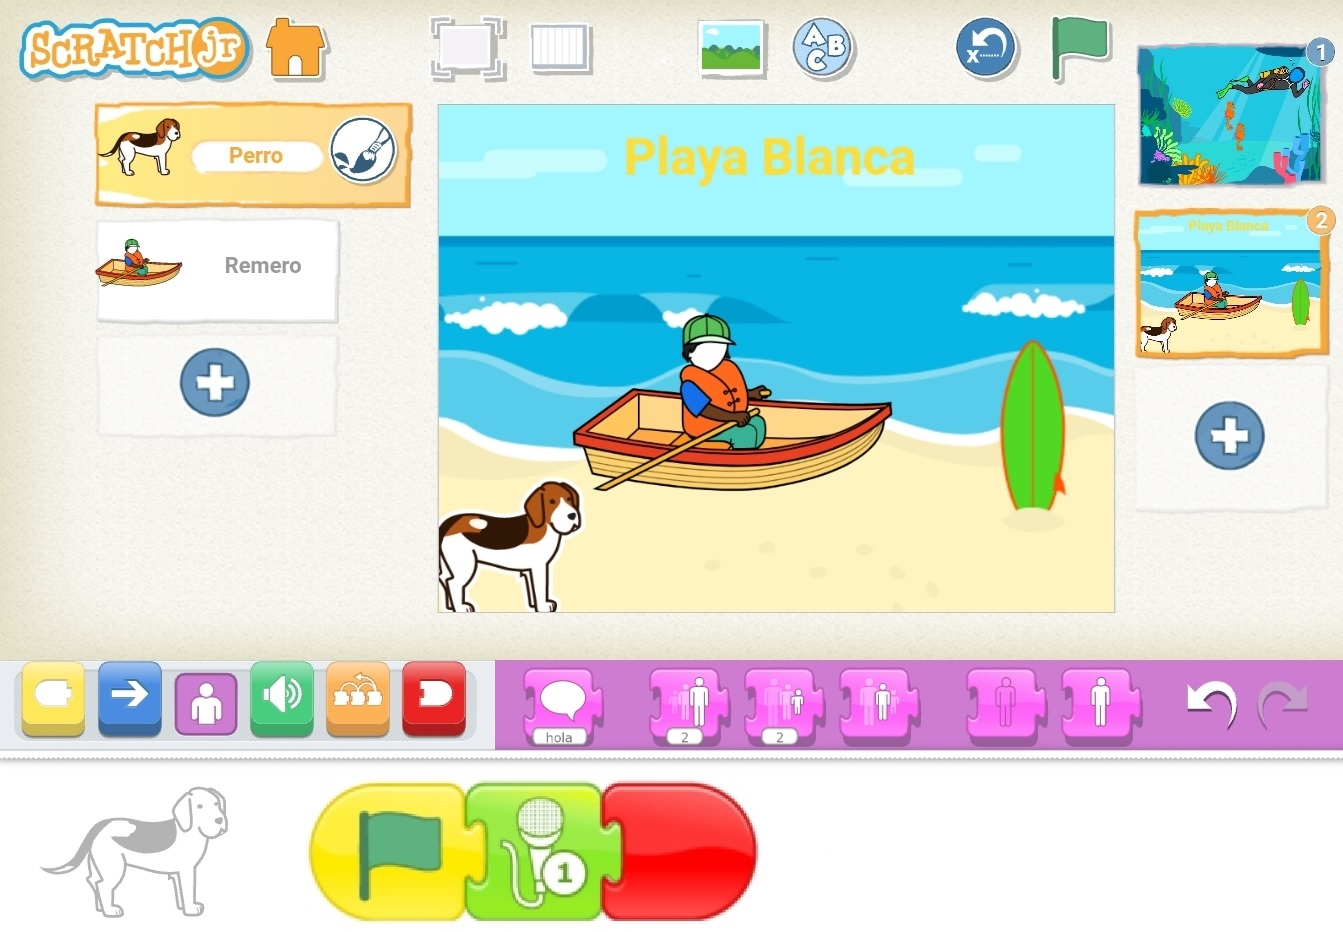
\includegraphics[width=0.48\textwidth]{img/perro_test.jpg}}
  \vspace{6mm}
   \subfloat[Remero]{
    \label{fig:remero}
     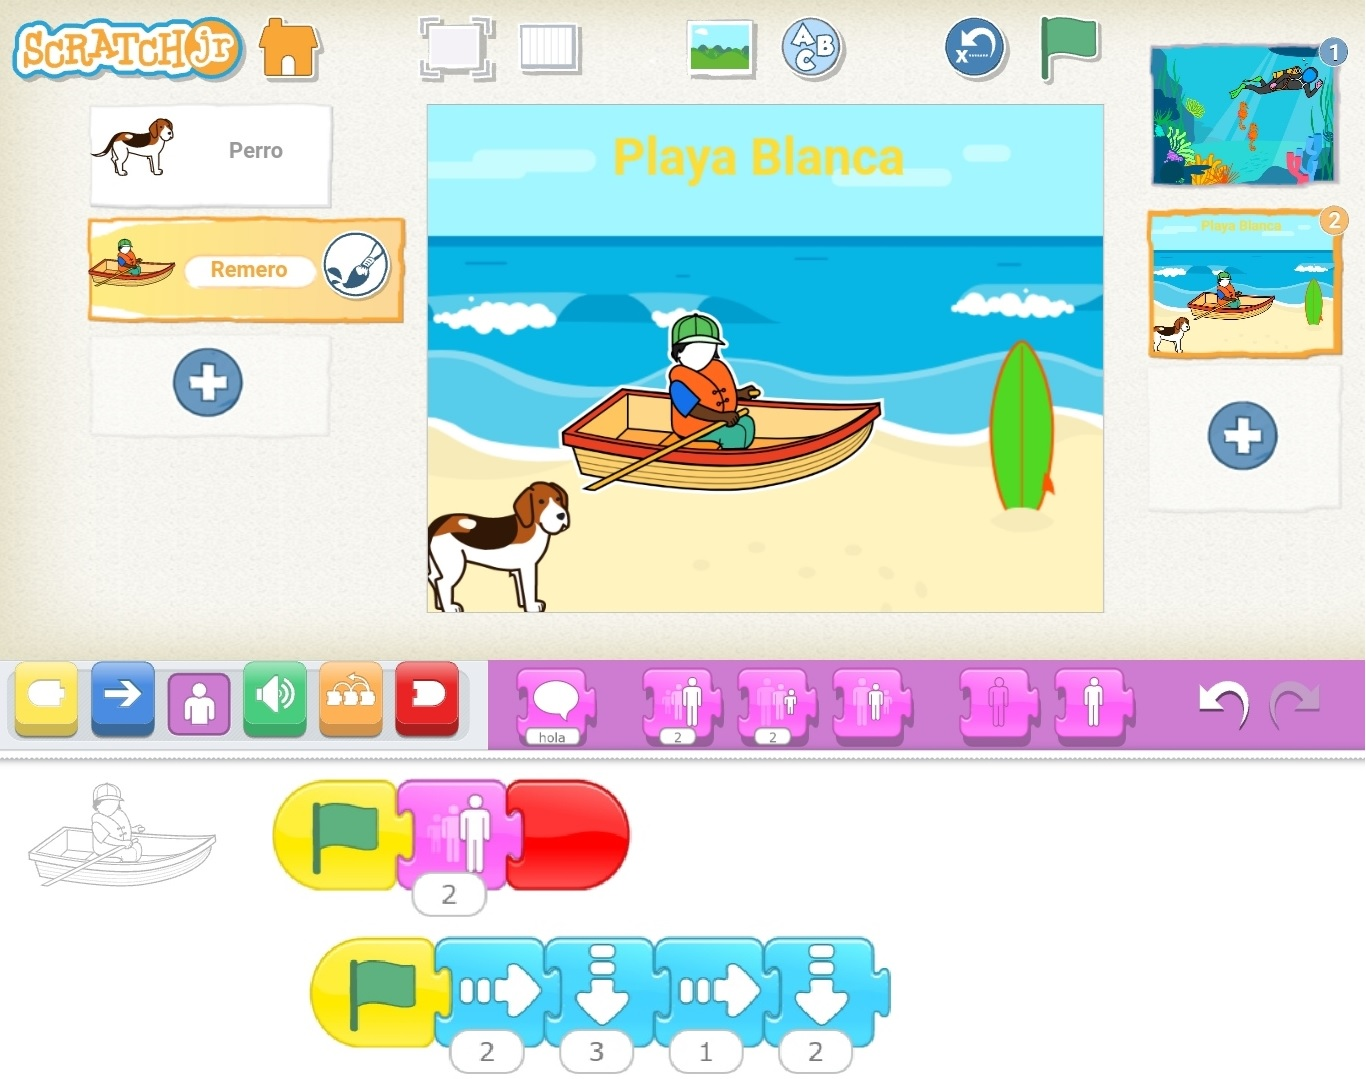
\includegraphics[width=0.52\textwidth]{img/remero_test.jpg}}
 \caption{Proyecto de ejemplo Test1.sjr} \label{fig:Test1}
\end{figure}


En la figura~\ref{fig:otros_datos_Test1} confirmamos estos datos con los mostrados en el análisis de Dr.ScratchJr.

\begin{figure}[H]
  \centering
  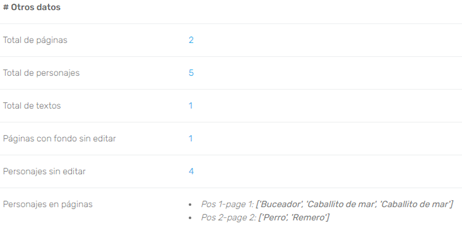
\includegraphics[width=14cm, keepaspectratio]{img/otros_datos_Test1.png}
  \caption{Otros datos del analisis de Test1.sjr.}
  \label{fig:otros_datos_Test1}
\end{figure}

\newpage

\begin{figure}[H]
Para validar el aspecto de Variabilidad hacemos un recuento de las ocasiones que aparece cada tipo de bloque en todo el proyecto (figura~\ref{fig:tabla_recuento}):\newline

  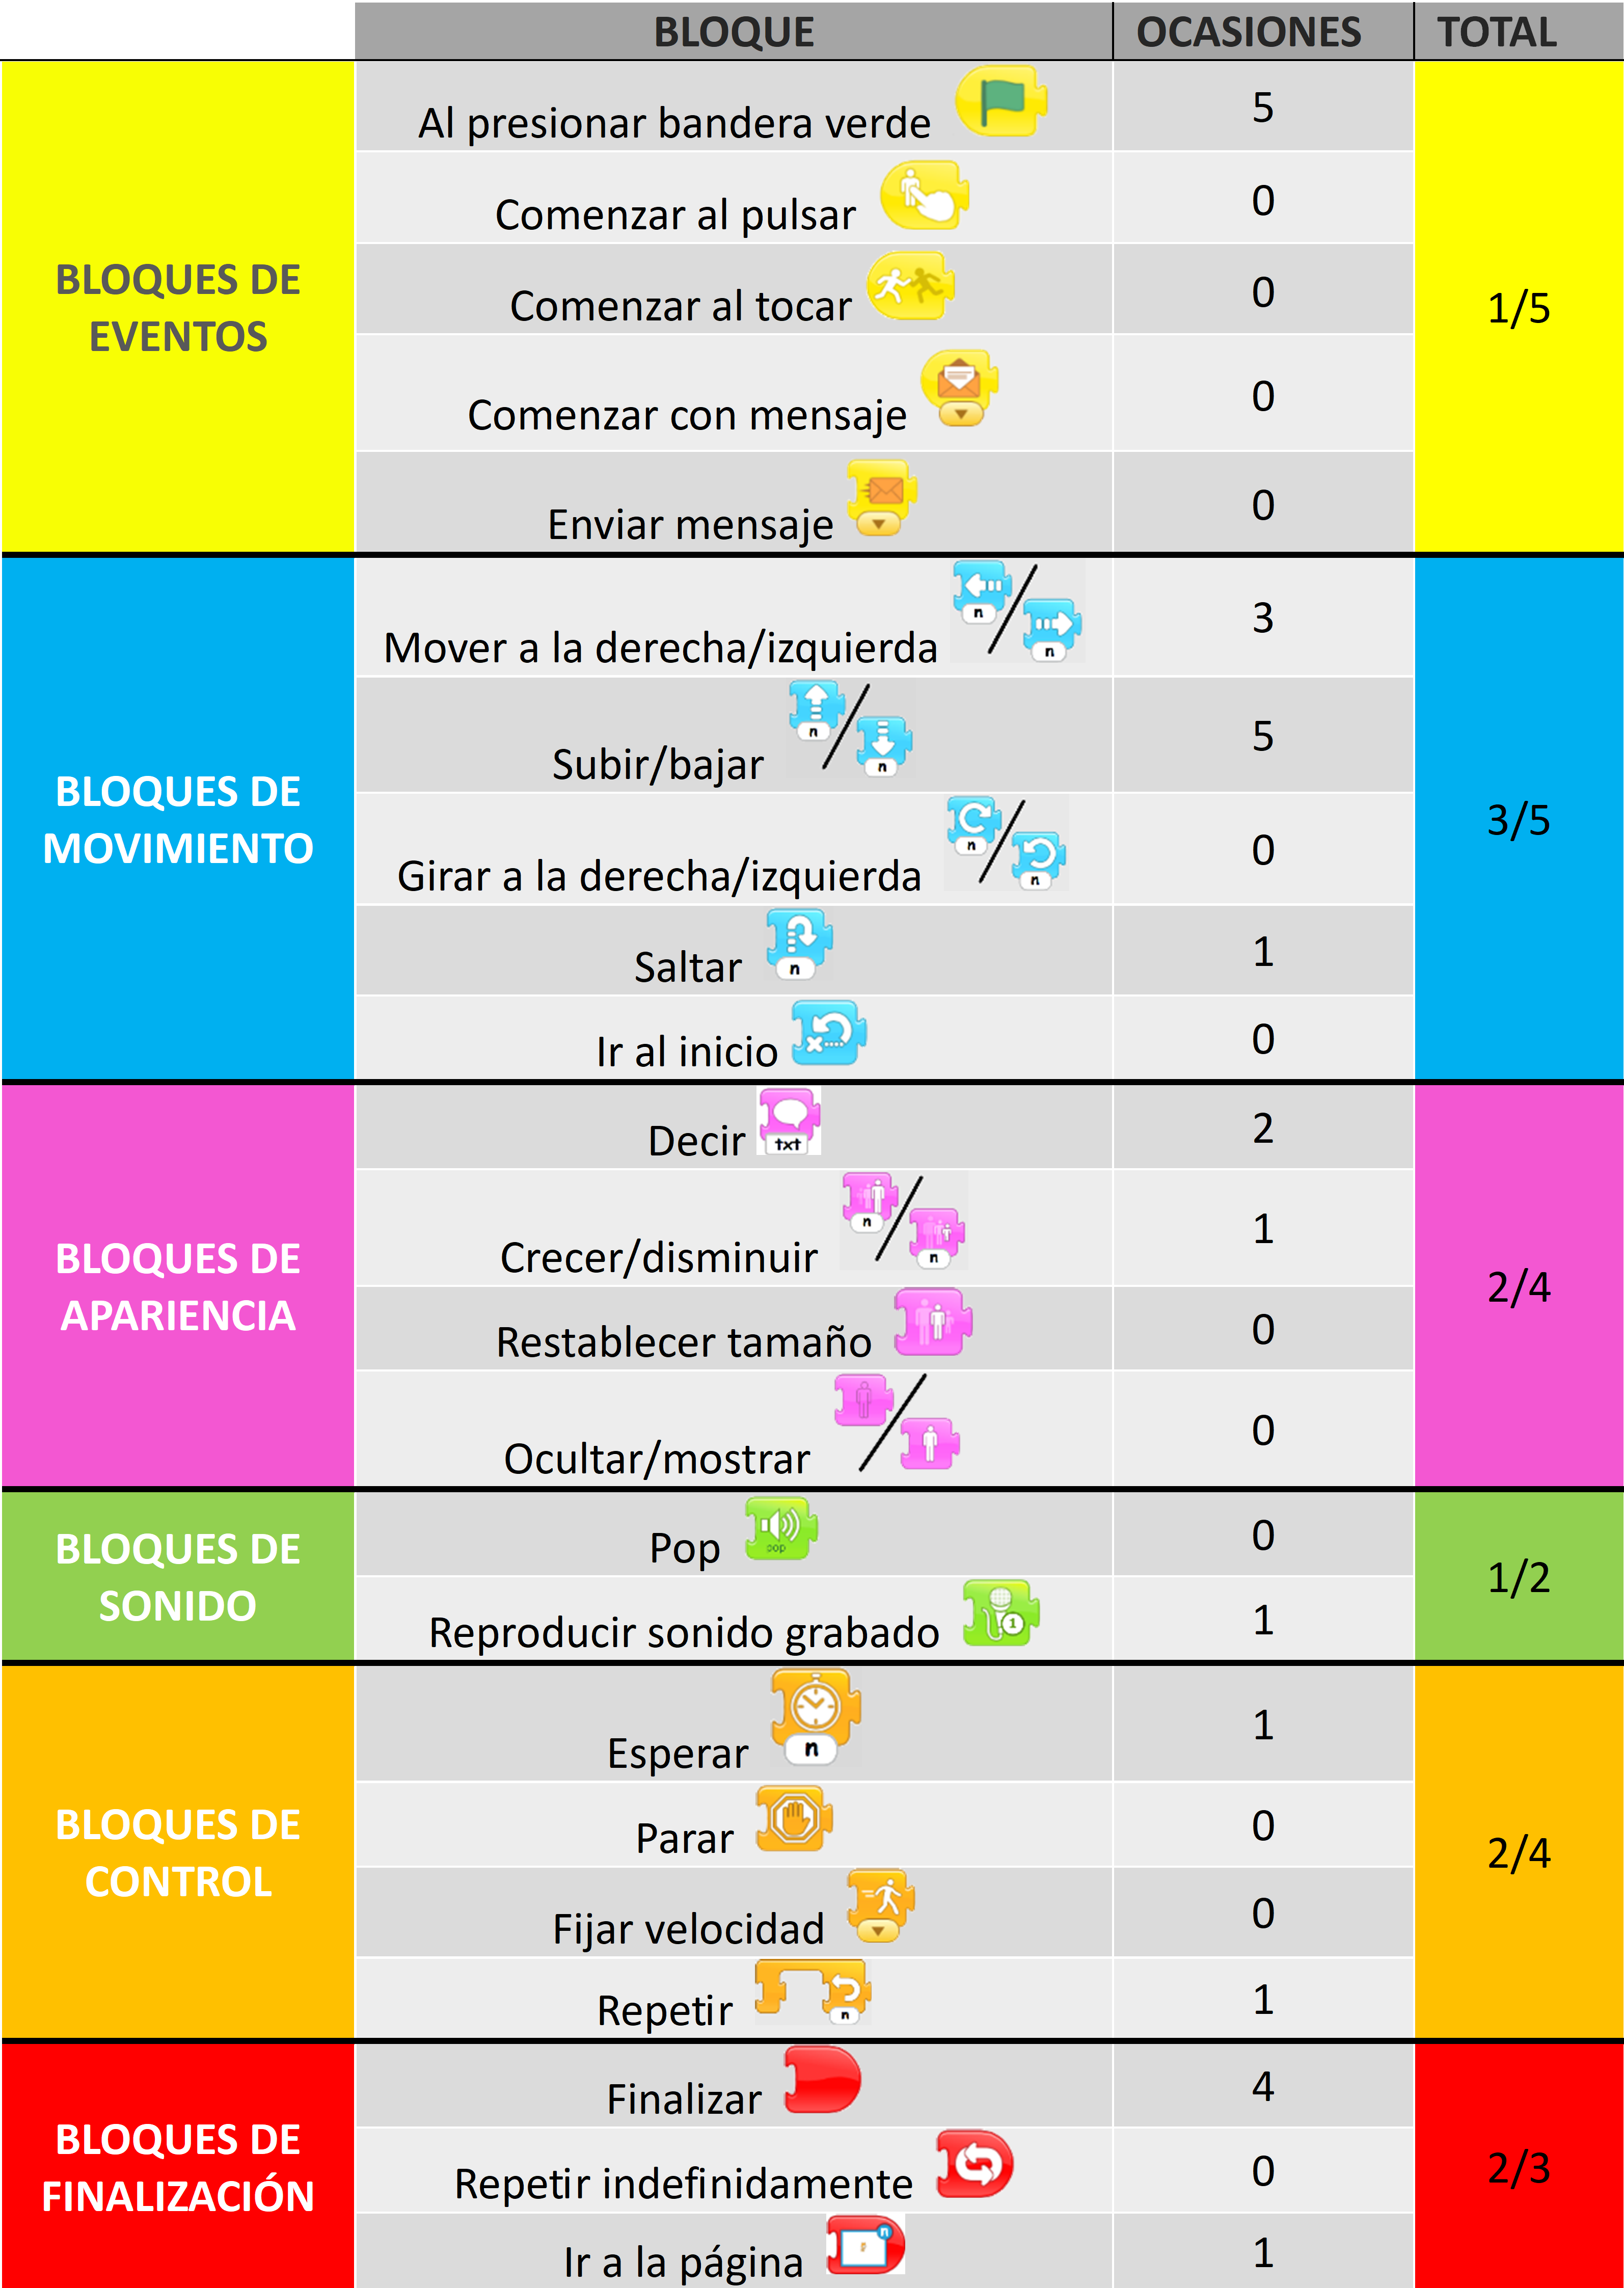
\includegraphics[width=15cm, keepaspectratio]{img/tabla_recuento.png}\centering
  \caption{Recuento total de bloques de Test1.sjr.}
  \label{fig:tabla_recuento}
\end{figure}

Comparando los resultados con el análisis del aspecto de Variabilidad de Dr.ScratchJr que se muestra en la figura~\ref{fig:variabilidad_Test1}, confirmamos que coinciden.

\begin{figure}[H]
  \centering
  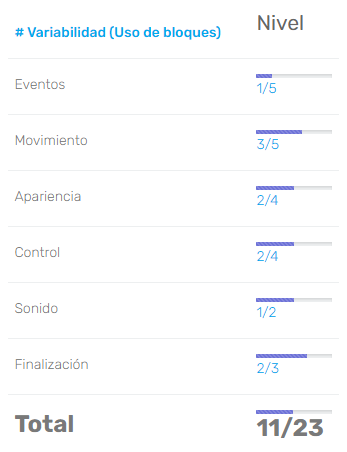
\includegraphics[ keepaspectratio]{img/variabilidad_Test1.png}
  \caption{Variabilidad del análisis de Test1.sjr.}
  \label{fig:variabilidad_Test1}
\end{figure}

Consideramos código muerto a secuencias de bloques que no se van a ejecutar en un proyecto porque no comienzan con un bloque de evento.
En nuestro ejemplo Test1.sjr, hay una secuencia de bloques donde ocurre esto.
En la figura~\ref{fig:caballito2} el personaje Caballito de mar posee una secuencia de bloques donde no se encuentra ningún bloque de evento, por lo tanto, no se va a realizar dicha secuencia y se considera que el proyecto contiene un \textit{Código muerto}.

\vspace{5mm}
Por el contrario, una secuencia de bloques que no acaba con un bloque de finalización se considera \textit{Código inacabado}. Es el caso que ocurre en una de las secuencias de la figura~\ref{fig:remero}.

\vspace{5mm}
En la figura~\ref{fig:caballito1}, aparecen dos bloques ``subir'' seguidos en una misma secuencia.
Esto se considera un mal hábito de \textit{Secuencias con bloques adyacentes} porque ScratchJr posee ciertos bloques que disponen de un atributo que representa el número de veces que quieres que se realicen dichos bloques de forma consecutiva sin la necesidad de estar repitiéndolos en el programa.

\vspace{5mm}
Otro mal hábito es el uso de \textit{Personajes con mismo nombre en una página}. En la página 1 de Test1.sjr (figura~\ref{fig:Test1}) aparecen dos personajes con el nombre Caballito de mar, por lo que este nombre se encuentra en la página 1 en dos ocasiones.


Los resultados del análisis del aspecto de Malos hábitos coinciden con lo esperado (figura~\ref{fig:maloshabitos_Test1}).

\begin{figure}[H]
  \centering
  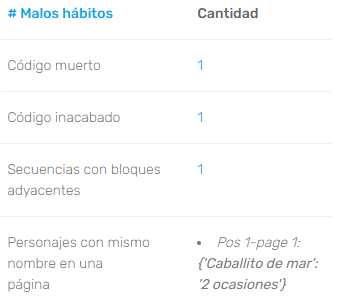
\includegraphics[keepaspectratio]{img/maloshabitos_Test1.png}
  \caption{Malos hábitos del análisis de Test1.sjr.}
  \label{fig:maloshabitos_Test1}
\end{figure}

De las dos páginas que tiene el proyecto Test1.sjr, la página 2 ha sido modificada con el editor de ScratchJr. Podemos ver en la figura~\ref{fig:pagina_editada} como la tabla de surf era de color naranja en el fondo de página que proporciona ScratchJr por defecto, y ahora es verde.
De tal manera el personaje ``Buceador'' ha sido editado cambiando de color los guantes y la máscara (figura~\ref{fig:personaje_editado}), siendo éste el único personaje que ha sido modificado.

\begin{figure}[H]
 \centering
  \subfloat[Personaje editado]{
   \label{fig:personaje_editado}
    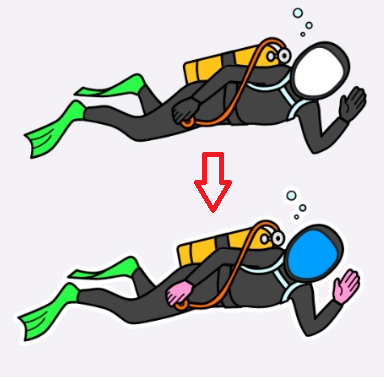
\includegraphics[width=0.35\textwidth]{img/personaje_editado.png}}
    \hfill
  \subfloat[Página editada]{
   \label{fig:pagina_editada}
    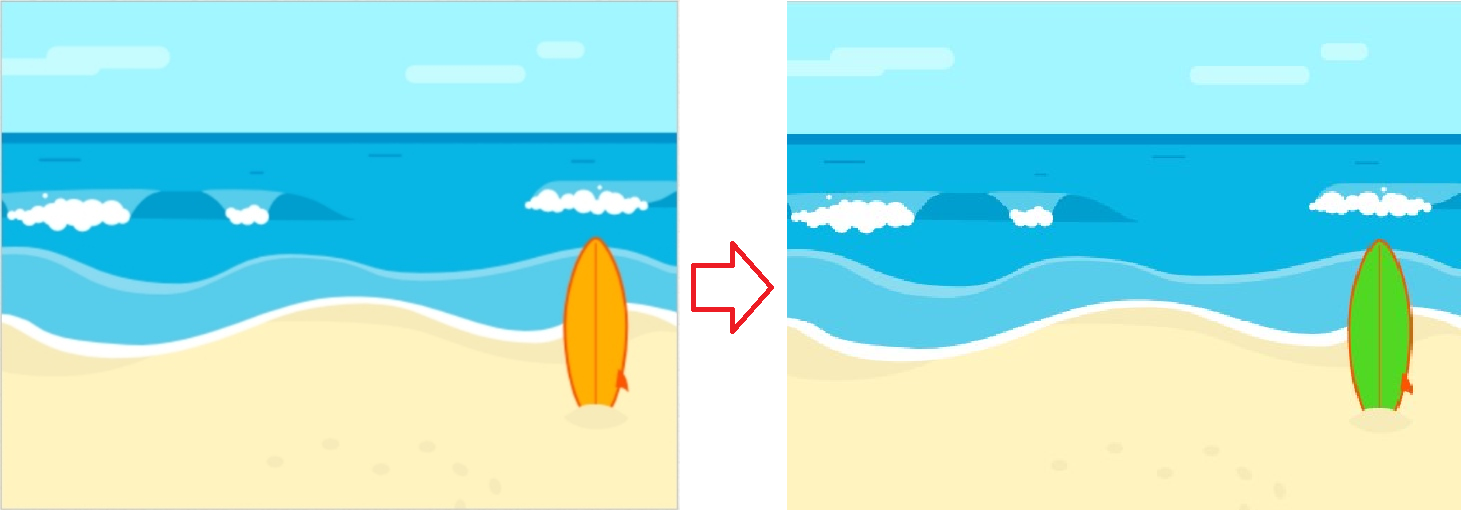
\includegraphics[width=0.60\textwidth]{img/pagina_editada.png}}
 \caption{Personaje y página editada de Test1.sjr} \label{fig:editados}
\end{figure}

En cuanto a sonidos creados, Test1.sjr contiene un bloque en la secuencia que tiene el personaje ``Perro'' de la página 2, con una grabación de audio emulando el sonido de la onomatopeya de ladridos.

\vspace{5mm}
Por último y para validar completamente el análisis de Dr.ScratchJr, los resultados del aspecto de Creatividad (figura~\ref{fig:creatividad_Test1}) también concuerdan con lo esperado.

\begin{figure}[H]
  \centering
  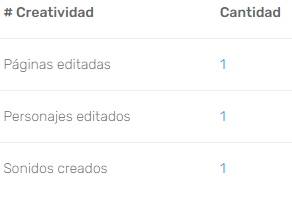
\includegraphics[keepaspectratio]{img/creatividad_Test1.png}
  \caption{Creatividad del análisis de Test1.sjr.}
  \label{fig:creatividad_Test1}
\end{figure}

\section{Cargar varios proyectos}
\label{sec:Cargar zip}

Ahora vamos a comprobar la funcionalidad de cargar varios proyectos simultáneamente en la aplicación.
Los archivos de los proyectos se comprimen en un zip y éstos deben estar nombrados con la estructura ``\textbf{`Nombre del proyecto'}-\textbf{`Nombre del estudiante'}.sjr'' para poder almacenarlos y asociarlos a sus autores correctamente en la aplicación.
Para ello usamos como ejemplo cuatro proyectos con los nombres modificados como se ha comentado anteriormente y almacenados en un zip llamado ``Test\_zip''. (figura~\ref{fig:Test_zip0}). 

\begin{figure}[H]
  \centering
  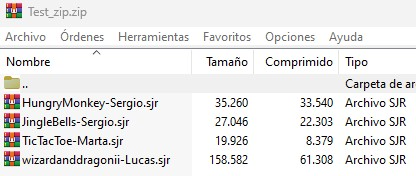
\includegraphics[keepaspectratio]{img/Test_zip0.jpg}
  \caption{Contenido del archivo Test\_zip.zip.}
  \label{fig:Test_zip0}
\end{figure}

Una vez cargado el zip y opcionalmente cambiado internamente en la aplicación el nombre de los proyectos o de los autores, aparece un listado como en la figura~\ref{fig:Test_zip} y donde comprobamos que se han cargado correctamente los proyectos para la posterior visualización del análisis de cada uno de ellos o exportando todos los análisis en formato CSV.

\begin{figure}[H]
  \centering
  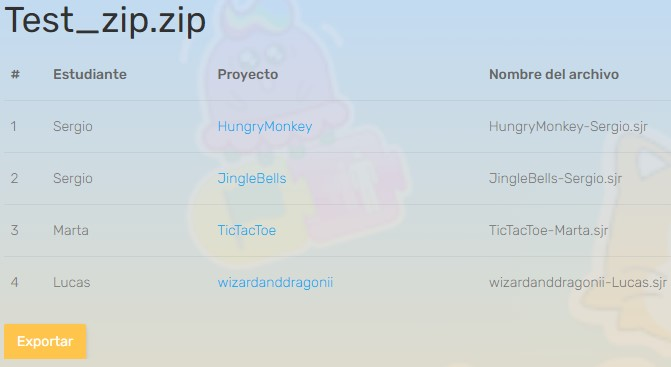
\includegraphics[keepaspectratio]{img/Test_zip.jpg}
  \caption{Listado de proyectos de Test\_zip en Dr.ScratchJr}
  \label{fig:Test_zip}
\end{figure}

\newpage
\section{Exportar datos en CSV}
\label{sec:exportarCSV}

Si se cargan varios proyectos a la vez a través de un zip o si se ha iniciado sesión y están almacenados los proyectos, Dr.ScratchJr tiene la opción de exportar los análisis de los proyectos.
En la figura~\ref{fig:Test1_csv}, vemos como se exportan correctamente en tres ficheros CSV distintos los datos del análisis del proyecto del ejemplo anterior Test1.sjr. 
Aunque también se exportan estos mismos datos en un archivo Excel dividido en pestañas.


\begin{figure}[H]
 \centering
  \subfloat[Variabilidad en formato CSV]{
   \label{fig:variabilidad_csv}
    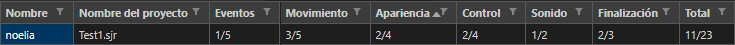
\includegraphics[width=0.98\textwidth]{img/variabilidad_csv.jpg}}
    \vspace{7mm}
  \subfloat[Otros datos en formato CSV]{
   \label{fig:otros_datos_csv}
    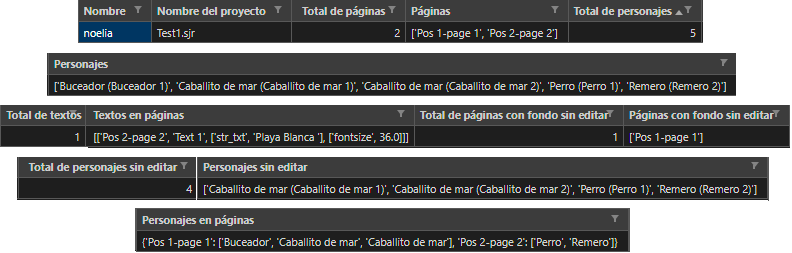
\includegraphics[width=0.98\textwidth]{img/otros_datos_csv.png}}
    \vspace{7mm}
  \subfloat[Malos hábitos en formato CSV]{
   \label{fig:maloshabitos_csv}
    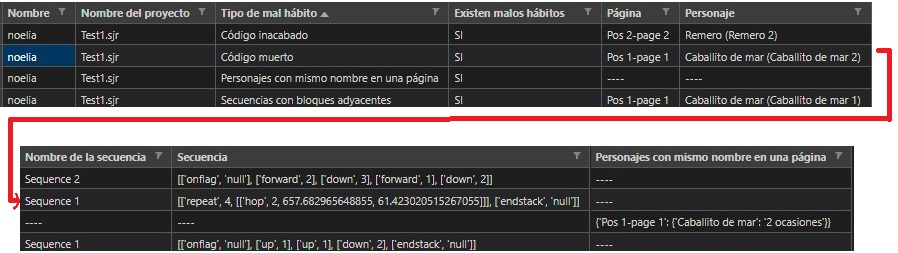
\includegraphics[width=0.98\textwidth]{img/maloshabitos_csv.jpg}}
 \caption{Datos en CSV del análisis de Test1.sjr} \label{fig:Test1_csv}
\end{figure}

%%%%%%%%%%%%%%%%%%%%%%%%%%%%%%%%%%%%%%%%%%%%%%%%%%%%%%%%%%%%%%%%%%%%%%%%%%%%%%%%
%%%%%%%%%%%%%%%%%%%%%%%%%%%%%%%%%%%%%%%%%%%%%%%%%%%%%%%%%%%%%%%%%%%%%%%%%%%%%%%%
% CONCLUSIONES %
%%%%%%%%%%%%%%%%%%%%%%%%%%%%%%%%%%%%%%%%%%%%%%%%%%%%%%%%%%%%%%%%%%%%%%%%%%%%%%%%

\cleardoublepage
\chapter{Conclusiones}
\label{chap:conclusiones}


\section{Consecución de objetivos}
\label{sec:consecucion-objetivos}

Los objetivos de este trabajo final de grado se han cumplido. 
Se ha creado una herramienta dónde se analizan proyectos de ScratchJr. 
Profesores o padres pueden subir a la aplicación web uno o varios proyectos simultáneamente de sus alumnos o hijos, ver el análisis de cada uno, almacenar y/o exportar los datos de los análisis.

\section{Aplicación de lo aprendido}
\label{sec:aplicacion_aprendido}

La mayoría de asignaturas que he cursado durante el Grado En Ingeniería En Sistemas Audiovisuales y Multimedia me han ayudado para la realización de este trabajo, puesto que me han ido formando en diversos aspectos, pero destacan:

\begin{itemize}
    \item Expresión Oral y Escrita y Búsqueda de Información porque me ha ayudado a redactar, buscar información y desarrollar la memoria.
    \item Informática I donde gracias al lenguaje de introducción a la programación ``Picky'' comencé a programar y aprender los fundamentos y las sintaxis básicas de la programación. 
    \item Informática II con el lenguaje Ada me ayudó a conocer mejor la programación, a cometer menos errores y a enfrentarme a proyectos un poco más complejos. 
    \item Protocolos para la Transmisión de Audio y Vídeo en Internet pues gracias a esta asignatura comencé con el lenguaje Python que se usa en este proyecto y que junto a Arquitectura de Internet y Sistemas Telemáticos para Medios Audiovisuales aprendí los conceptos de arquitectura de red y protocolos, así como los métodos de interconexión de redes y encaminamiento, ayudándome a utilizar los fundamentos de la programación en internet.
    \item Construcción de Servicios y Aplicaciones Audiovisuales en Internet ya que aprendí desarrollo web del lado del cliente y que me ha servido para usar HTML, CSS y JavaScript en el proyecto.
    \item Laboratorio de Tecnologías Audiovisuales en la Web es la asignatura que más me ha servido para poder realizar mi proyecto porque  es donde aprendí más sobre las tecnologías web para la construcción de aplicaciones y servicios.
    Y donde adquirí los conocimientos para utilizar Django como tecnología web en el lado del servidor y los mecanismos de interacción entre cliente y servidor.
\end{itemize}

\section{Lecciones aprendidas}
\label{sec:lecciones_aprendidas}

Realizar este trabajo final de grado ha sido un gran reto y un verdadero quebradero de cabeza. 
Nunca me había enfrentado a un proyecto tan amplio y complejo partiendo de cero.
La mayoría de prácticas del Grado han estado guiadas y esquematizadas, teniendo gran parte de la información necesaria disponible para realizarlas y obviamente han sido mucho más breves sin requerir de tanta elaboración.

\vspace{5mm}
He aprendido, aunque tarde, ha organizar mi propio tiempo y enfrentarme a los problemas y solucionarlos.
Durante el grado, siempre había unas fechas para realizar los exámenes y entregar trabajos que me empujaban y obligaban a esforzarme, y como durante la realización de este proyecto no tenia ninguna presión del tiempo, en cuanto me surgía cualquier problema me estancaba, lo dejaba pasar y volver a retomar el proyecto se me tornaba más complicado. 
Pero al final conseguí compaginar el trabajo con el proyecto y aprovechar más el tiempo.

\vspace{5mm}
Gracias a este proyecto he aprendido a elaborar una aplicación web completa, a manejar el código, las funciones, la base de datos, los archivos…para que todo tenga una estructura ordenada y enlazada. Por supuesto afianzando y ampliando todo lo estudiado en las asignaturas del Grado mencionadas en sección anterior~\ref{sec:aplicacion_aprendido}.

\vspace{5mm}
También a la hora de realizar la memoria he aprendido a plasmar y redactar todo el trabajo realizado y era algo que no estaba habituado a ello.

\section{Trabajos futuros}
\label{sec:trabajos_futuros}

Puesto que es una aplicación web necesitará de contante mantenimiento y, siendo mi primera, de numerosas correcciones.

En cuanto a ampliar las funcionalidades de Dr.ScratchJr se podría:
\begin{itemize}
    \item Mejorar el análisis de los proyectos añadiendo más criterios que den mayor información.
    \item Añadir otra función a la aplicación donde un usuario pueda ver estadísticas de todos los análisis que tenga almacenados y así tener mayor control e información.
    \item Crear otro apartado dónde haya enunciados de ejercicios específicos para hacer proyectos de ScratchJr con distintos niveles de dificultad y dónde Dr.ScratchJr evalúe con una nota si se ha realizado correctamente en exclusiva dicho ejercicio. 
    Un ejemplo de ejercicio sería uno donde se tenga que hacer un proyecto contando una historia en ciertos lugares, que contenga ciertos personajes y que usen mínimo ciertos bloques.
\end{itemize}


%%%%%%%%%%%%%%%%%%%%%%%%%%%%%%%%%%%%%%%%%%%%%%%%%%%%%%%%%%%%%%%%%%%%%%%%%%%%%%%%
%%%%%%%%%%%%%%%%%%%%%%%%%%%%%%%%%%%%%%%%%%%%%%%%%%%%%%%%%%%%%%%%%%%%%%%%%%%%%%%%
% APÉNDICE(S) %
%%%%%%%%%%%%%%%%%%%%%%%%%%%%%%%%%%%%%%%%%%%%%%%%%%%%%%%%%%%%%%%%%%%%%%%%%%%%%%%%

\cleardoublepage
\appendix
\chapter{Manual de usuario}
\label{app:manual}

La aplicación web Dr.ScratchJr\footnote{\url{http://spereztfg.pythonanywhere.com/}} se encuentra desplegada en el servicio de alojamiento web Pythonanywhere.

Pero además se puede instalar en local, donde mejoran considerablemente los tiempos de carga de los análisis.
Para ello es necesario:

\begin{enumerate}
    \item Descargar los archivos del repositorio de Github\footnote{\url{https://github.com/sperezmaz/Dr.ScratchJr.git}}
    \item Tener instalado Python 3.9, Django 3.1.3, Django-Registration 3.1.1, Pandas 1.2.4 y Openpyxl 3.0.7.
    \item Aunque no sea necesario para realizar el análisis de un proyecto, para configurar un servidor de correo propio, en el fichero settings.py situado en la carpeta descargada drscratchjr hay que cambiar los valores de las siguientes variables:
        \begin{itemize}
            \item EMAIL\_HOST: servidor SMTP que se utilizará para enviar correos electrónicos.
            \item EMAIL\_HOST\_USER: nombre de usuario que se utilizará para el servidor SMTP.
            \item EMAIL\_HOST\_PASSWORD: contraseña que se utilizará para el servidor SMTP.
            \item EMAIL\_PORT: puerto que se utilizará para el servidor SMTP.
        \end{itemize}
    \item Abrir el terminal en el directorio donde se encuentre el archivo manage.py y ejecutar los comandos:
        \begin{itemize}
            \item \begin{verbatim}python manage.py makemigrations\end{verbatim}
            \item \begin{verbatim}python manage.py migrate\end{verbatim}
            \item \begin{verbatim}python manage.py runserver\end{verbatim}
        \end{itemize}
    \item Abrir en un navegador la siguiente URL:
    \begin{center}
        \url{http://127.0.0.1:8000}
    \end{center}
    
\end{enumerate}

Ya sea en local o en Pythonanywhere, para analizar un proyecto ScratchJr sin almacenar su análisis en la aplicación web solo se debe encontrar en la página de inicio el formulario llamado ``Analizar proyecto'', darle al botón ``Seleccionar archivo'', buscar el proyecto deseado y pulsar sobre ``Analizar''.
Por el contrario, si se quiere almacenar los resultados se debe crear una cuenta y posteriormente iniciar sesión.
La única diferencia, en el formulario ``Analizar proyecto'' cuando se ha iniciado sesión, es que en el momento de subir el proyecto se necesita asociar dicho proyecto a un estudiante existente o crear uno nuevo escribiendo su nombre.

Si se desea analizar varios proyectos a la vez y exportar los resultados, en la página de inicio aparece otro formulario llamado ``Analizar varios proyectos'', en el que se debe subir un archivo .zip donde están comprimido todos los proyectos que se quieren analizar nombrados ``NombreProyecto-NombreEstudiante.sjr''.
Al pulsar sobre analizar debe aparecer una página con otro formulario pre-rellenado por si se quiere modificar el nombre del proyecto o del estudiante.
Cuando se pulsa en el botón finalizar se muestra una lista de los proyectos subidos en los que pinchando en el nombre del proyecto podemos ver su análisis.
En esta lista existe la opción de descargar los resultados de los análisis dándole al botón exportar.
Igualmente, para almacenar los análisis en la aplicación era necesario haber iniciado sesión previamente. 

Para más detalles, dos vídeos explicativos del funcionamiento de la aplicación web Dr.ScratchJr:
\begin{itemize}
    \item Para utilizar la aplicación sin registrarse.\footnote{\url{https://www.youtube.com/watch?v=wAnI3-UCVCs}}
    \item Para utilizar la aplicación con las ventajas de tener un usuario.\footnote{\url{https://www.youtube.com/watch?v=ZXXOl7qqiMw}}
\end{itemize}

%%%%%%%%%%%%%%%%%%%%%%%%%%%%%%%%%%%%%%%%%%%%%%%%%%%%%%%%%%%%%%%%%%%%%%%%%%%%%%%%
%%%%%%%%%%%%%%%%%%%%%%%%%%%%%%%%%%%%%%%%%%%%%%%%%%%%%%%%%%%%%%%%%%%%%%%%%%%%%%%%
% BIBLIOGRAFIA %
%%%%%%%%%%%%%%%%%%%%%%%%%%%%%%%%%%%%%%%%%%%%%%%%%%%%%%%%%%%%%%%%%%%%%%%%%%%%%%%%

\cleardoublepage

% Las siguientes dos instrucciones es todo lo que necesitas
% para incluir las citas en la memoria
\bibliographystyle{abbrv}
\bibliography{memoria}  % memoria.bib es el nombre del fichero que contiene
% las referencias bibliográficas. Abre ese fichero y mira el formato que tiene,
% que se conoce como BibTeX. Hay muchos sitios que exportan referencias en
% formato BibTeX. Prueba a buscar en http://scholar.google.com por referencias
% y verás que lo puedes hacer de manera sencilla.
% Más información: 
% http://texblog.org/2014/04/22/using-google-scholar-to-download-bibtex-citations/

\end{document}
